\chapter{รายละเอียดการปฏิบัติงาน}
\thispagestyle{empty}
\label{chapter:coop-detail}

\section{ตำแหน่ง/หน้าที่ของงานที่ได้รับมอบหมาย}

    \subsection{ตำแหน่งงาน}
        PROGRAMMER
    
    \subsection{หน้าที่ของงานที่ได้รับมอบหมาย}
        \begin{enumerate}
            \item ศึกษาวิธีการทดสอบกับ Flutter แอปพลิเคชันโดยการเพิ่ม key
            \item ศึกษาวิธีการใช้งาน Appium ซึ่งเป็น Framework ที่ช่วยในการทดสอบ แอปพลิเคชัน อัตโนมัติ
            \item ศึกษาวิธีการใช้งาน Appium กับ Flutter ผ่าน Flutter Appium Driver Library
            \item ศึกษาการใช้งาน AWS Device Farm ซึ่งเป็นตัวช่วยจำลองโทรศัพท์ในการทดสอบแอปพลิเคชัน
            \item ศึกษาการพัฒนาชุดคำสั่งทดสอบด้วย NodeJs
            \item ศึกษา HomePro E-Catalog แอปพลิเคชนซึ่งเป็นแอปพลิเคชันที่ต้องนำมาทดสอบ
            \item ออกแบบและพัฒนาชุดคำสั่งทดสอบ
            \item จัดทำคู่มือวิธีการติดตั้ง Appium, AWS Device Farm, NodeJs
            \item จัดทำคู่มือวิธีการพัฒนาชุดคำสั่งทดสอบอัตโนมัติด้วย NodeJs กับ Flutter Appium Driver Library
            \item จัดทำคู่มือวิธีการใช้งาน Appium, AWS Device Farm, NodeJs
        \end{enumerate}

\section{รายละเอียดของโครงงานที่ได้รับผิดชอบ}

    เนื่องจากใน {\Company} เป็นบริษัทขนาดใหญ่จึงจำเป็นต้องมีแอปพลิเคชันหรือระบบภายในไว้ใช้งานจึงมีแผนก ICT Non SAP Front Office
    ไว้คอยพัฒนาระบบหรือแอปพลิเคชันโดยในการจะนำเอาแอปพลิเคชันมาใช้งานหรือแก้ไขต้องเกิดการทดสอบก่อนเสมอเพื่อลดข้อผิดพลาดทางแผนกจึงมอบหมายงาน
    ให้พัฒนาการทดสอบแอปพลิเคชันอัตโนมัติ (Automate Testing) ของแอปพลิเคชัน HomePro E-Catalog ที่เป็นแอปพลิเคชันที่สร้างขึ้นด้วย Flutter เพื่อเป็นต้นแบบไว้คอยนำมาประยุกต์ใช้งานกับ
    แอปพลิเคชันที่จะเกิดขึ้นในอนาคต โดยงานหลักแบ่งได้ 2 อย่างได้แก่
    
    \begin{enumerate}
        \item พัฒนาชุดคำสั่งทดสอบไว้ใช้กับแอปพลิเคชัน HomePro E-Catalog ควบคู่กับ AWS Device Farm
        \item จัดทำเอกสารคู่มือการติดตั้ง, การใช้งาน AWS Device Farm, วิธีการพัฒนาชุดคำสั่งทดสอบ
    \end{enumerate}

    \subsection{ขอบเขตของโครงการ}
        จัดทำชุดคำสั่งทดสอบอัตโนมัติกับแอปพลิเคชันที่ถูกสร้างขึ้นมาด้วย Flutter โดยจะสามารถทดสอบในระบบ Android ได้เท่านั้น โดยกรณีศึกษาจากแอปพลิเคชัน HomePro E-Catalog
        โดยสามรถแบ่งการทดสอบเป็น 34 เหตุการณ์โดยสามารถแบ่งดังนี้
        
        \quad 1. การเขียนทดสอบด้วยกรจับ Element บนหน้าจอโดยไม่ต้องแก้ไขที่ Source Code โดยแบ่งเป็นหน้าจอดังนี้
            \begin{itemize}
                \item หน้าจอ Log-in
                \item หน้าจอ ออกจากระบบ
                \item หน้าจอ รายละเอียดสินค้า
                \item หน้าจอ เปรียบเทียบสินค้า
                \item หน้าจอ รถเข็นสินค้า
                \item หน้าจอ หมวดผู้ใช้งาน
                \item หน้าจอ หมวดเมนู
            \end{itemize}

        \quad 2. การเขียนการทดสอบด้วยการจับ แก้ไขที่ Source Code ของ Flutter โดยใช้ Appium Flutter Driver โดยแบ่งตามหน้าจอดังนี้
            \begin{itemize}
                \item หน้าจอ หมวดสินค้า (Level 3)
                \item หน้าจอ หมวดหมู่ย่อย (Level 2)
                \item หน้าจอ หมวดหมู่ย่อย (Level 1)
            \end{itemize}

        เมื่อพัฒนาชุดคำสั่งเสร็จสิ้นจึงนำไปทดสอบบน AWS Device Farm และจัดทำเอกสารคู่มือวิธีการติดตั้ง, วิธีการพัฒนาชุดคำสั่งทดสอบ, คู่มือการใช้งาน AWS Device Farm

\newpage
\section{รายละเอียดของงานที่ปฏิบัตินอกเหนือจากโครงการที่รับผิดชอบ}
    นอกเหนือจากงานโครงการที่ได้รับผิดชอบยังมีงานอื่นในการช่วยการทำงานของแผนกในฐานะ PROGRAMMER โดยสามารถแบ่งโปรเจ็คที่ได้ทำเป็น 2 ประเภทได้แก่
    
    \subsection{บริการระบบงานขาย Single Sale}
        เป็นระบบที่ใช้ในการยืนยันการซื้อขายสินค้าโดยผู้ใช้งานจะเป็นพนักงานของสาขา {\Company} โดยงานที่ได้รับมอบหมายส่วนใหญ่คือการหาข้อผิดพลาดของระบบและทำการแก้ไข
        ยกตัวอย่าง เช่น การนำข้อมูลออกมาแสดงไม่ถูกต้องจึงต้องไปดูวิธีการนำข้อมูลออกมาและทำการแก้ไขให้ทำงานได้อย่างถูกต้อง หรือ ทำการสร้างหมวดย่อยใหม่เป็นประเภทในการสั่งซื้อสินค้าของลูกค้าเป็นต้น
    
    \subsection{ระบบงานจัดส่งและบริการ Delivery Service}
        เป็นระบบที่ใช้ในการสร้างและยืนยันปิดงานจัดส่งสินค้าโดยผู้ใช้งานจะเป็น พนักงานสาขา, พนักงานจัดส่ง, คอลเซ็นเตอร์ ของ {\Company} โดยงานที่ได้รับมอบหมายส่วนใหญ่คือการหาข้อผิดพลาดของระบบและทำการแก้ไข
        ยกตัวอย่าง เช่น การจัดทีมช่างไปที่บ้านลูกค้าแสดงไม่ถูกต้องจึงต้องทำการแก้ไขให้แสดงได้อย่างถูกต้อง หรือ การปิดงานบางครั้งเป็นงานต่อเนื่องทำหลายวัน
        แต่ระบบได้ปิดงานไปแล้วจึงต้องทำการแก้ไขให้สามารถเก็บการปิดงานเป็นรายวันได้

\section{ลักษณะขั้นตอนกํารทำงาน}
        ลักษณะขั้นตอนการทำงานเป็น รูปแบบ WaterFall มี step การทำอย่างชัดเจนโดยสามารถแบ่งการทำงานดังนี้

\section{ทฤษฎีที่เกี่ยวข้อง}
    \subsection{การทดสอบซอฟต์แวร์ (Software Testing)}
        Software Testing คือ การทดสอบว่าระบบทำงานได้อย่างถูกต้องหรือไม่ตามวัตถุประสงค์หรือเปล่าและสามารถระบุข้อผิดพลาดเพื่อสามารถนำไปแก้ไขได้
        ก่อนการนำไปจัดส่งซึงการทำการทดสอบซอฟต์แวร์นั้นมีความสำคัญมากเนื่องจากการเจอ ข้อผิดพลาดในซอฟต์แวร์นั้นมีค่าใช้จ่ายที่สูงหากเกิดขึ้นตอนนำจัดส่งไปแล้ว
        โดยการทดสอบซอฟต์แวร์แบ่งเป็นได้ 2 ประเภทได้แก่
        \begin{enumerate}
            \item Manual Testing คือ การทดสอบที่ไม่ใช้เครื่องมืออัตโนมัติหรือ Script เลยจะทดสอบตาม Test Plan, Test Case หรือ Test Scenarios ด้วยมือของผู้ทดสอบเอง
            \item Automation Testing คือ การทดสอบอัตโนมัติด้วยการเขียนชุดคำสั่งในการทดสอบ (Script)
        \end{enumerate}
        \begin{figure}[H]
            \centering
            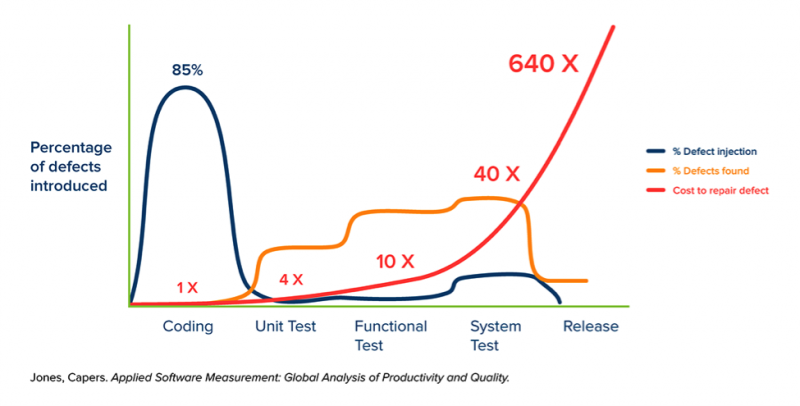
\includegraphics[width=1\textwidth]{cost-of-fixing-bug}
            \caption{ค่าใช้จ่ายการแก้ข้อผิดพลาดที่แปรผันตามขั้นตอนของการพัฒนาซอฟต์แวร์}\label{cost-of-fixing-bug}
        \end{figure}

    \subsection{การทดสอบอัตโนมัติ (Automation Testing)}
        Automation Testing คือ การทดสอบแบบอัตโนมัติโดยการเขียนชุดคำสั่งทดสอบแทนแบบเดิมที่ใช้การทดสอบก้วยมือ ยกตัวอย่าง เช่น
        การทดสอบซอฟต์แวร์แบบเดิมด้วยการใช้มือจะต้องกรอกแบบสอบถามในแอปพลิเคชันในวันแรกและเจอข้อผิดพลาดวันถัดไปนักพัฒนาแอปพลิเคชัน
        ก็ปรับปรุงแอปพลิเคชันมาใหม่ให้ไปทดสอบกรอกแบบเดิมอีกและอาจเจอข้อผิดพลาดใหม่หรือไม่เจอแต่ถ้าหากเกิดการแก้ไขหรือเปลี่ยนแปลงกับ
        ตัวแอปพลิเคชันแล้วต้องทำการทดสอบใหม่อยู่ตลอดซึ่งเป็นการทำงานรูปแบบเดิม แต่การทำ Automation Testing จะมาช่วยแก้ปัญหาโดย
        การเขียนชุดคำสั่งเพื่อมากรอกแบบทดสอบให้ในแอปพลิเคชันซึ่งกำหนดไว้ว่าสิ่งที่ถูกต้องควรจะเป็นอย่างไรและหากไม่ถูกต้องไม่ถูกต้องอย่างไร
        โดยจะเป็นการทำแบบอัตโนมัติด ดังนั้นข้อดีของ Automation Testing ได้แก่
        \begin{itemize}
            \item[-] ผลตอบรับที่ไวขึ้นต่อรอบการพัฒนาหรือแก้ไขแอปพลิเคชัน
            \item[-] สามารถประหยัดค่าใช้จ่ายในการทดสอบได้
            \item[-] สามารถทดสอบได้อย่างคลอบคลุมมากขึ้น
            \item[-] สามารถนำแอปพลิเคชันมาส่งมอบได้เร็วขึ้น
            \item[-] เพิ่มความแม่นยำในการทดสอบมากขึ้น 
            \item[-] กำจัดการทดสอบที่จะผิดพลาดที่เกิดจากมนุษย์ 
        \end{itemize}
        ในปัจจุบันมีเครื่องมือช่วยในการทำ Automation Testing มากมายยกตัวอย่างดังนี้
        \begin{enumerate}

            \item Katalon Studio คือ เครื่องมือตัวหนึ่งในการช่วยทำ Test Automation ของ Mobile Applications ซึ่งสามารถทดสอบได้ทั้ง
            Android และ IOS
            \begin{figure}[H]
                \centering
                
\includegraphics[width=0.3\textwidth]{katalon-studio}
                \caption{ตราตราสัญลักษณ์ Katalon Studio}\label{katalon-studio}
            \end{figure}

            \item Selenium คือ Software Testing Framework ที่มีประสิทธิภาพไว้ใช้สำหรับเขียนชุดคำสั่งทดสอบ Web Applications ซึ่งเป็นแบบ Open Source สามารถเขียนได้ด้วยหลายภาษา เช่น Java, Python, \texttt(C\#), Javascript, PHP, Perl 
            \begin{figure}[H]
                \centering
                
\includegraphics[width=0.5\textwidth]{selenium}
                \caption{ตราตราสัญลักษณ์ Selenium}\label{selenium}
            \end{figure}

            \item Micro Focus UFT คือ หนึ่งใน Software ที่มีประสิทธิภาพที่สุดสำหรับการทำการทดสอบแบบ Functional Testing สามารถสร้าง Test และแก้ไขได้อย่างรวดเร็วไปจนถึงสามารถนำเทคโนโลยี Object Recognition, Image-based Automation และ Machine Driven Regression Testing เข้ามาใช้ช่วยในการทำงาน
            แต่เสียค่าใช้จ่ายแต่มีให้ทดลองใช้งานฟรี 60 วัน
            \begin{figure}[H]
                \centering
                
\includegraphics[width=0.20\textwidth]{uft}
                \caption{ตราตราสัญลักษณ์ Micro Focus UFT}\label{uft}
            \end{figure}

            \item TestComplete คือ หนึ่งใน Software ที่มีประสิทธิภาพที่สุดสำหรับการทำการทดสอบ Desktop, Mobile และ Web Applications ตามชุดคำสั่งที่เขียนได้ด้วย
            ภาษา Python, JavaScript, VBScript และอื่นๆ
            \begin{figure}[H]
                \centering
                
\includegraphics[width=0.5\textwidth]{test-com}
                \caption{ตราตราสัญลักษณ์ TestComplete}\label{test-com}
            \end{figure}


        \end{enumerate}

    \subsection{Appium}
        Appium คือ เครื่องมือสำหรับการทำ Automation Testing เป็นรุปแบบ Open Source ไว้สำหรับทดสอบ Native, Mobile Web, Hybrid
        , Android, IOS และ Windows Desktop การใช้ Appium จะเป็น Cross Platform หมายความว่าจะทำให้สามารถเขียน
        โดยใช้ API เดียวกันซึ่งจะช่วยให้สามารถใช้โค้ดซ้ำระหว่างอุปกรณ์ที่ทดสอบได้ IOS, Android, Window การทำงานจะสื่อสารระหว่าง Driver กับ Appium ผ่าน JSON โดยรองรับการเขียนได้หลายภาษา
        เช่น Python, Java, JavaScript(NodeJS), Ruby 
        \begin{figure}[H]
            \centering
            
\includegraphics[width=0.3\textwidth]{appium}
            \caption{ตราตราสัญลักษณ์ Appium}\label{appium}
        \end{figure}

        Driver ที่สามารถใช้กับ Appium ได้แก่
        \begin{itemize}
            \item XCUITest Driver (for iOS and tvOS apps)
            \item Espresso Driver (for Android apps)
            \item UiAutomator2 Driver (for Android apps)
            \item Windows Driver (for Windows Desktop apps)
            \item Mac Driver (for Mac Desktop apps)
        \end{itemize}

        \begin{figure}[H]
            \centering
            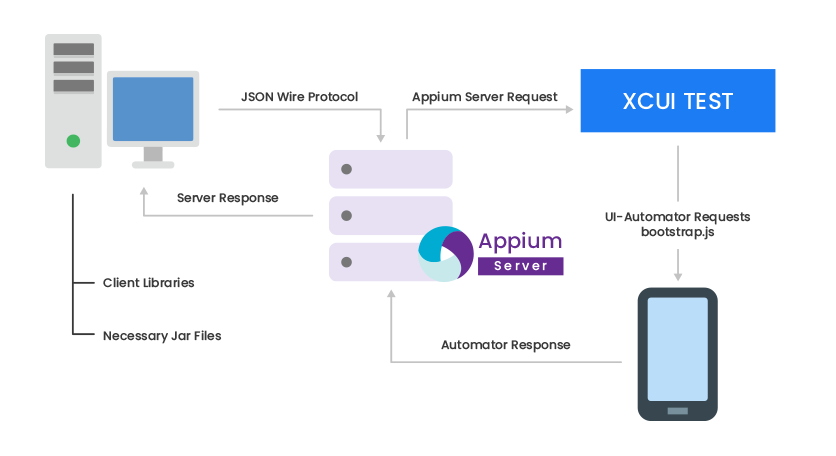
\includegraphics[width=1\textwidth]{appium-arc}
            \caption{โครงสร้างการทำงานของ Appium}\label{appium-arc}
        \end{figure}

        นอกเหนือจากนี้ Appium ยังสามารถใช้งานร่วมกับ AWS Device Farm ได้

    \subsection{API}
        API (Application Programming Interface) คือ วิธีการติดต่อสื่อสารระหว่างแอปพลิเคชันไม่ว่าแอปพลิเคชันนั้นจะรันอยู่บนอุปกรณ์ใด เช่นคอมพิวเตอร์ โทรศัพท์มือถือ หรือเฟิร์มแวร์ในอุปกรณ์เครื่องใช้ต่างๆ โดยที่แอปพลิเคชันฝั่งหนึ่งเป็นผู้ขอใช้บริการหรือขอข้อมูลจากแอปพลิเคชันอีกฝั่งหนึ่งซึ่งเป็นผู้ให้บริการ การติดต่อสื่อสารระหว่างแอปพลิเคชันดังกล่าวเป็นไปโดยอัตโนมัติตามที่ได้กำหนดไว้

    \subsection{AWS Device Farm}
         AWS คือ Amazon Web Services เป็นคลาวด์แพลตฟอร์มที่มีคนนำมาใช้มากที่สุดในโลกที่มีการบริการ 175 บริการ
         โดยองค์กรขนาดใหญ่หรือสตาร์ทอัพก็เริ่มหันมาใช้ AWS เพื่อลดค่าใช้จ่ายและความคล่องตัว

        \begin{figure}[H]
            \centering
            
\includegraphics[width=0.5\textwidth]{aws}
            \caption{ตราสัญลักษณ์ Amazon Web Service (AWS)}\label{aws}
        \end{figure}

        AWS Device Farm คือ บริการหนึ่งของ AWS เป็นบริการไว้ทดสอบแอปพลิเคชันเพื่อปรับปรุงคุณภาพแอปพลิเคชันหรือระบบต่างๆ
        โดย AWS Device Farm จะทดสอบแอปพลิเคชันหรือระบบใน Desktop, Browser หรืออุปกรณ์มือถือที่หลากหลายทั้งในระบบปฎิบัติการ Android และ IOS พร้อมกันเพื่อช่วย
        ให้ชุดทดสอบรวดเร็วขึ้น หลากหลายมากขึ้น และพร้อมสร้างวีดีโอและบันทึกเพื่อช่วยให้หาปัญหาของระบบหรือแอปพลิเคชันได้ไวยิ่งขึ้น

        \begin{figure}[H]
            \centering
            
\includegraphics[width=0.25\textwidth]{amazon-device-farm}
            \caption{ตราสัญลักษณ์ AWS Device Farm}\label{amazon-device-farm}
        \end{figure}

    \subsection{Node.Js}
        Node.Js คือ JavaScript runtime environment เป็น OpenSource คือการที่สามารถนำเอา JavaScript มาใช้งานแบบภาษาอื่นบน
        Windows, Linux หรือ Mac ได้แบบไม่เสียค่าใช้จ่ายหากติดตั้ง Node.js จะสามารถเขียนโปรแกรมด้วยภาษา JavaScript เหมือนกับ Java, \texttt(C\#), Python
        ซึ่งหลักๆแล้วจะนำมาทำเป็น backend server นอกจากนี้ Node.Js ยังมี NPM (Node Package Manager) เป็นตัวที่ใช้สำหรับการดาวน์โหลด
        library ภายนอกมาใช้โดยติดตั้งเพียงพิมพ์ `npm install <ชื่อ library>` เช่น mocha, express, chai เป็นต้น

        \begin{figure}[H]
            \centering
            
\includegraphics[width=0.3\textwidth]{node}
            \caption{ตราสัญลักษณ์ Node.JS}\label{node}
        \end{figure}
        

    \subsection{Flutter}
        Flutter คือ Framework แบบ OpenSource ที่ถูกพัฒนาโดย Google มีไว้เพื่อใช้สร้าง UserInterface สำหรับ Mobile Application ที่สามารถทำงานข้ามแพลตฟอร์มได้ทั้ง IOS และ Android คือเขียนโปรแกรมหนึ่งครั้งสามารถนำมาใช้ได้ทั้งสองแพลตฟอร์มโดยภาษาที่ Flutter ใช้คือภาษา Dart
        โดยจุดเด่นของ Flutter คือระบบ Hot Reload จะเข้ามาช่วยในส่วนของการ reload สามารถพัฒนาแอปพลิเคชัน ในส่วน UserInterface มีความรวดเร็วมากขึ้นอีกทั้งยังมีความสวยงามแบบ
        Material Design

        \begin{figure}[H]
            \centering
            
\includegraphics[width=0.5\textwidth]{flutter}
            \caption{ตราสัญลักษณ์ Flutter}\label{flutter}
        \end{figure}

    \subsection{Appium Flutter Driver}
        Appium Flutter Driver คือ เครื่องมือช่วยในการทำ Automation Test กับแอปพลิเคชันที่สร้างมาจาก Flutter เป็นส่วนหนึ่งในการใช้งานกับ Appium โดย Appium Flutter Driver จะใช้ Dart Service Protocol เพื่อส่ง API ไปเรียกใช้การ Test ของ Flutter ที่ทั่วไปต้องเขียนเป็นภาษา Dart แต่ถ้าใช้ library นี้จะเขียนภาษาตามที่ Appium มีได้เลย

        \begin{figure}[H]
            \centering
            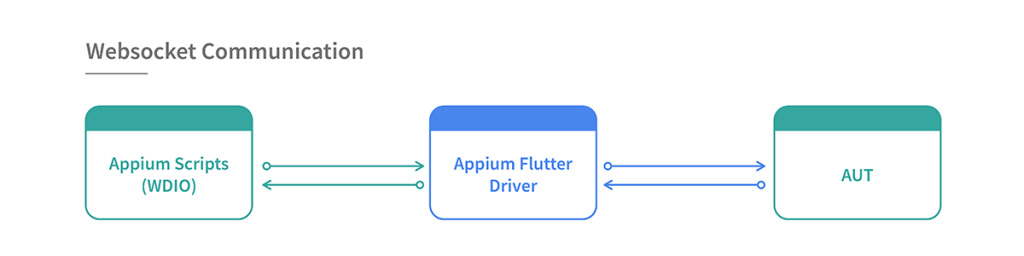
\includegraphics[width=1\textwidth]{appium-flutter}
            \caption{โครงสร้างการทำงานของ Appium Flutter Driver}\label{appium-flutter}
        \end{figure}

    \subsection{WebdriverIO}
        WebdriverIO คือ library JavaScript ที่ใช้ในการทำ Automation Test ใน NodeJS โดยที่สามารถทำงานร่วมกับ Selenium และ Appium ได้
        
    \subsection{Mocha}
        Mocha คือ library JavaScript ที่ใช้ใน NodeJs เพื่อทำการทดสอบอัตโนมัติแบบ Asynchronous Testing ได้ง่ายขึ้นโดยการแสดงผลลัพธ์ที่ผิดพลาดอย่างง่ายและชัดเจนตาม Test Case

    \subsection{Chai}
        Chai คือ library JavaScript ที่ใช้ใน NodeJs ทำหน้าที่เปรียบที่ค่าผลลัพธิ์ที่ได้จากการทดสอบกับผลลัพธ์ที่ควรจะเป็นโดยเป็นรูปแบบที่เข้าใจง่าย

    \subsection{Git}
        Git คือ Vesion Control เป็นตัวที่ใช้จัดเก็บและคอยดูการเปลี่ยนแปลงกับไฟล์ชนิดใดก็ได้เมื่อจัดเก็บไฟล์เข้าไปในระบบของ Git แล้วจะเรียกว่า Git Repository ซึ่งสำรองข้อมูลของ Source Code สามารถย้อนกลับไปเวอร์ชั่นใดก่อนหน้าและดูรายละเอียดการเปลี่ยนแปลงของแต่ละเวอร์ชั่นได้

        \begin{figure}[H]
            \centering
            
\includegraphics[width=0.3\textwidth]{git-logo}
            \caption{ตราสัญลักษณ์ Git}\label{git-logo}
        \end{figure}

    \subsection{Visual Studio Code}
        Visual Studio Code คือ Editor ตัวหนึ่งที่สร้างมาเพื่ออำนวยความสะดวกแก่โปรแกรมเมอร์มีธีมและรองรับรูปแบบการเขียนได้หลายภาษาอีกทั้งยังมีตัวช่วยในการเขียนโปรแกรมต่างๆ เช่น Bracket Matcher, Live Server เป็นต้น

        \begin{figure}[H]
            \centering
            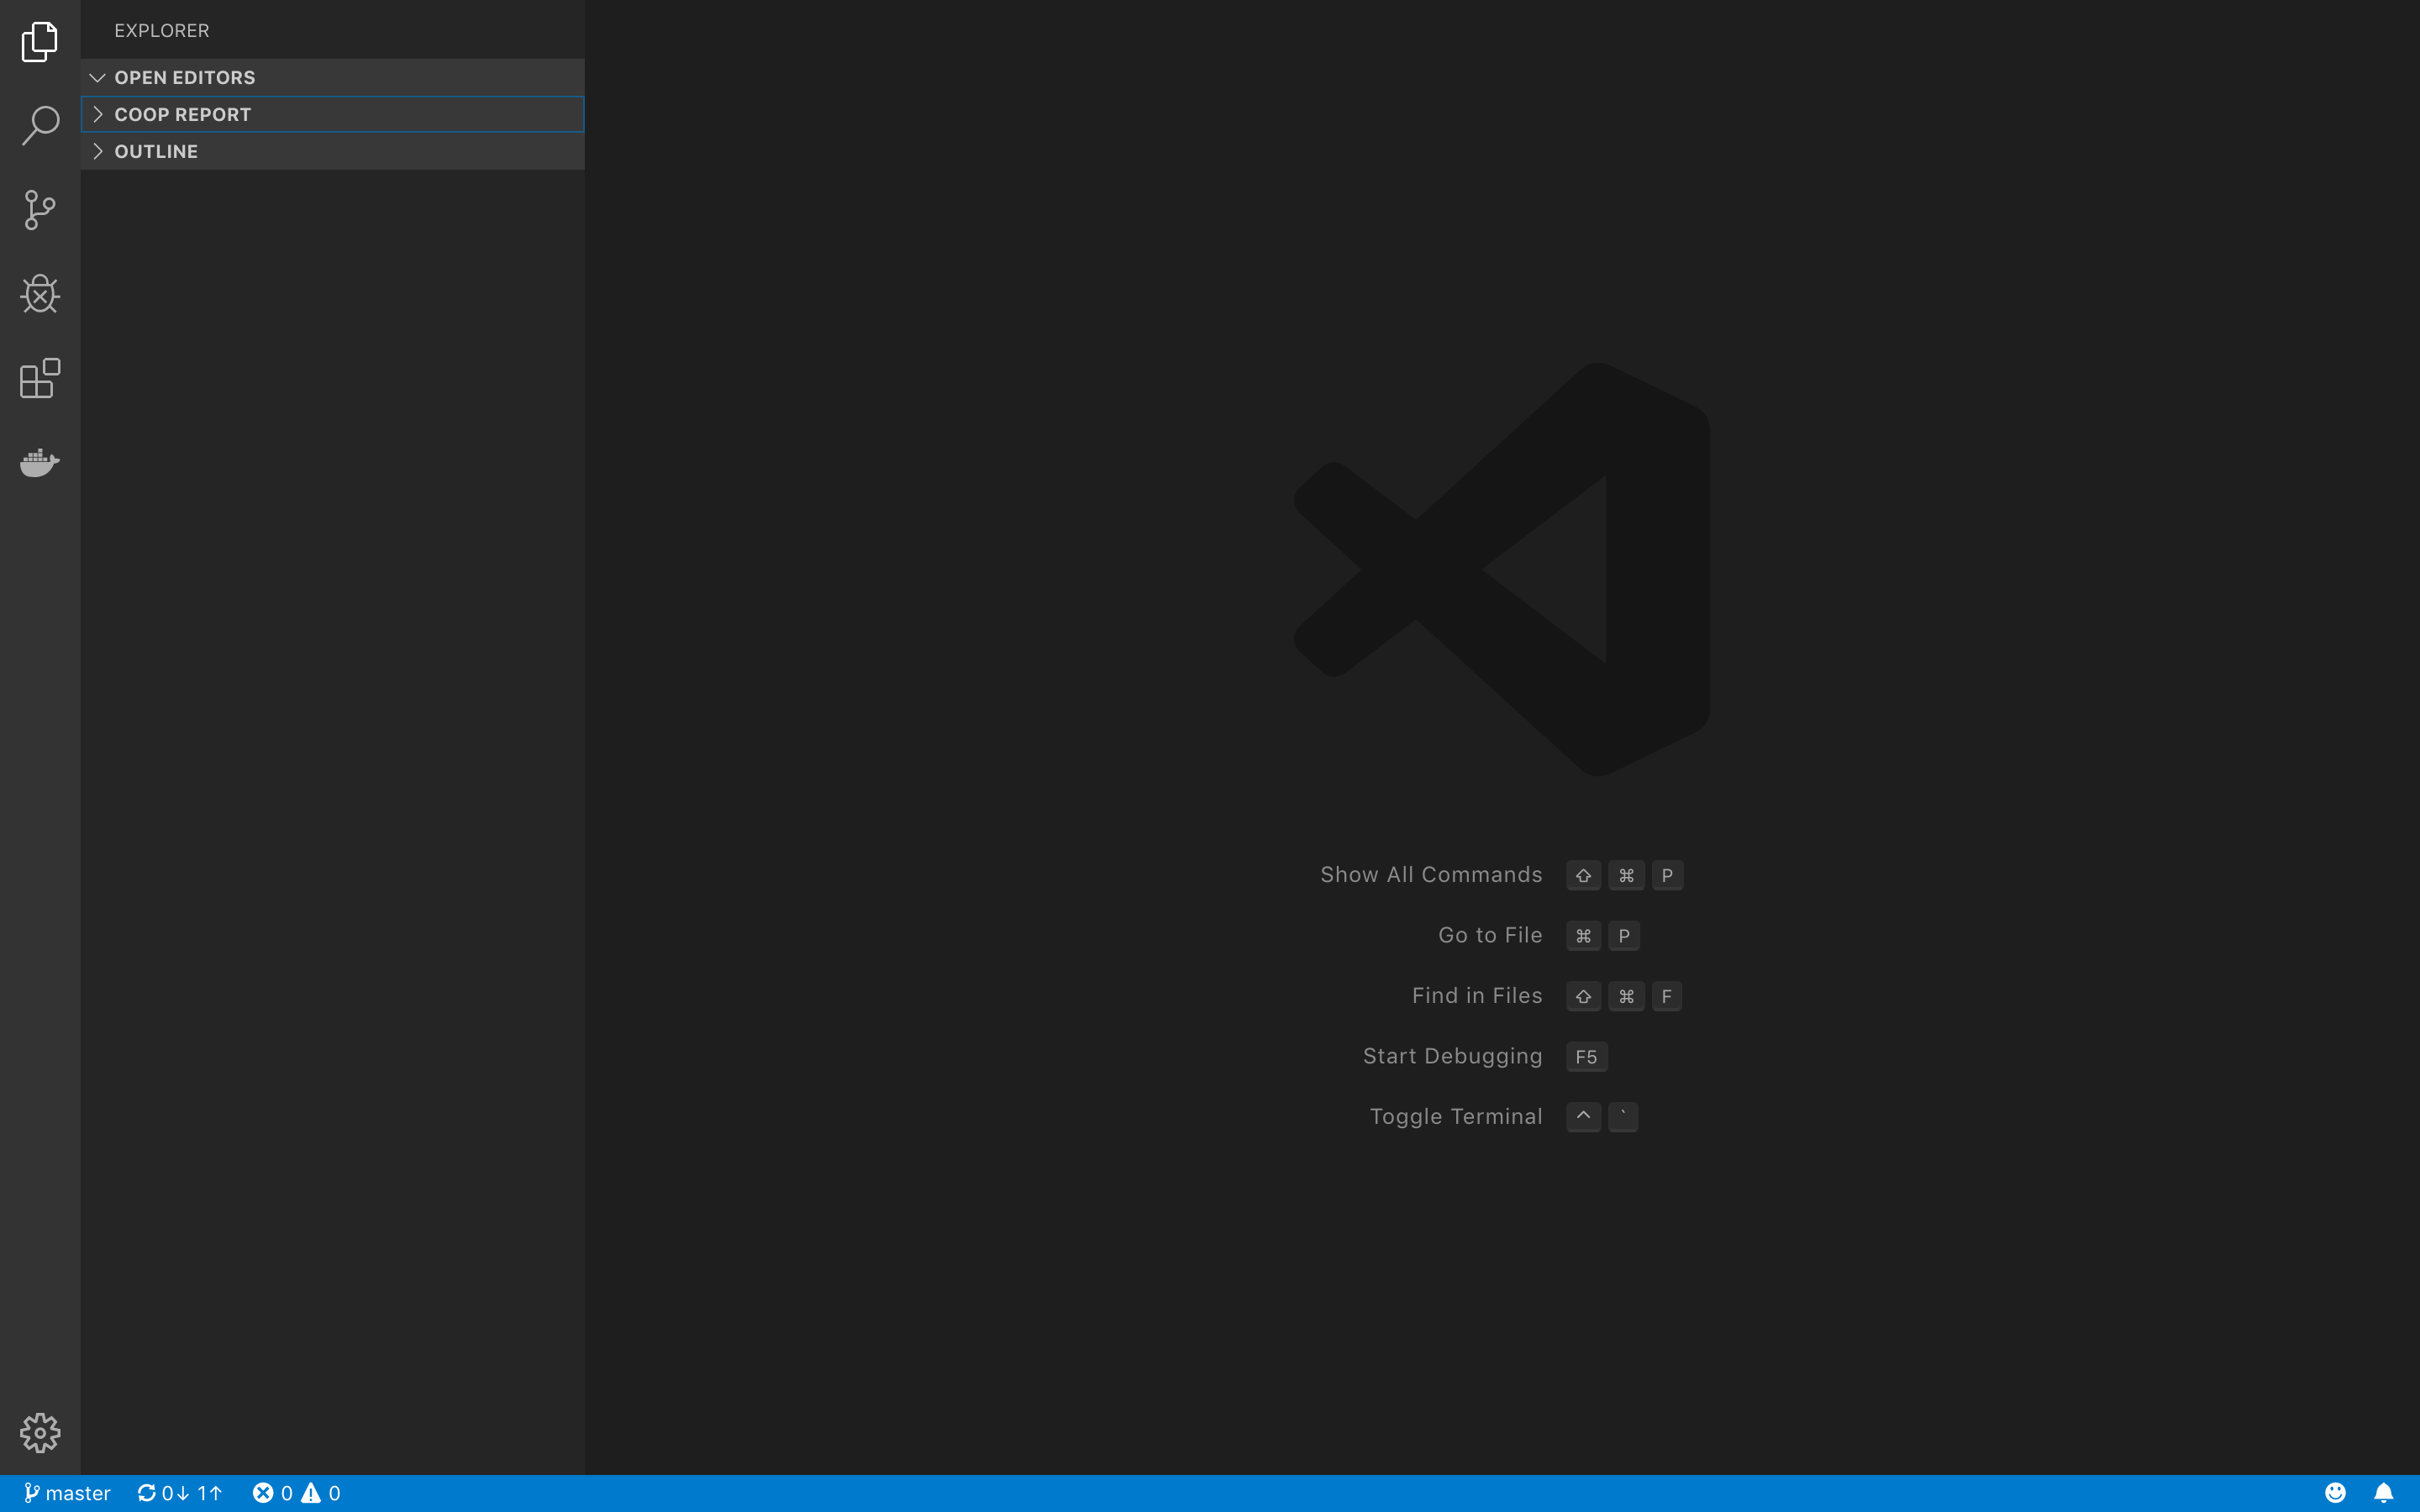
\includegraphics[width=0.2\textwidth]{visual-studio-code}
            \caption{ตราสัญลักษณ์ Visual Studio Code}\label{visual-studio-code}
        \end{figure}


%     \subsection{VIP}
%         \begin{figure}[H]
%             \centering
%             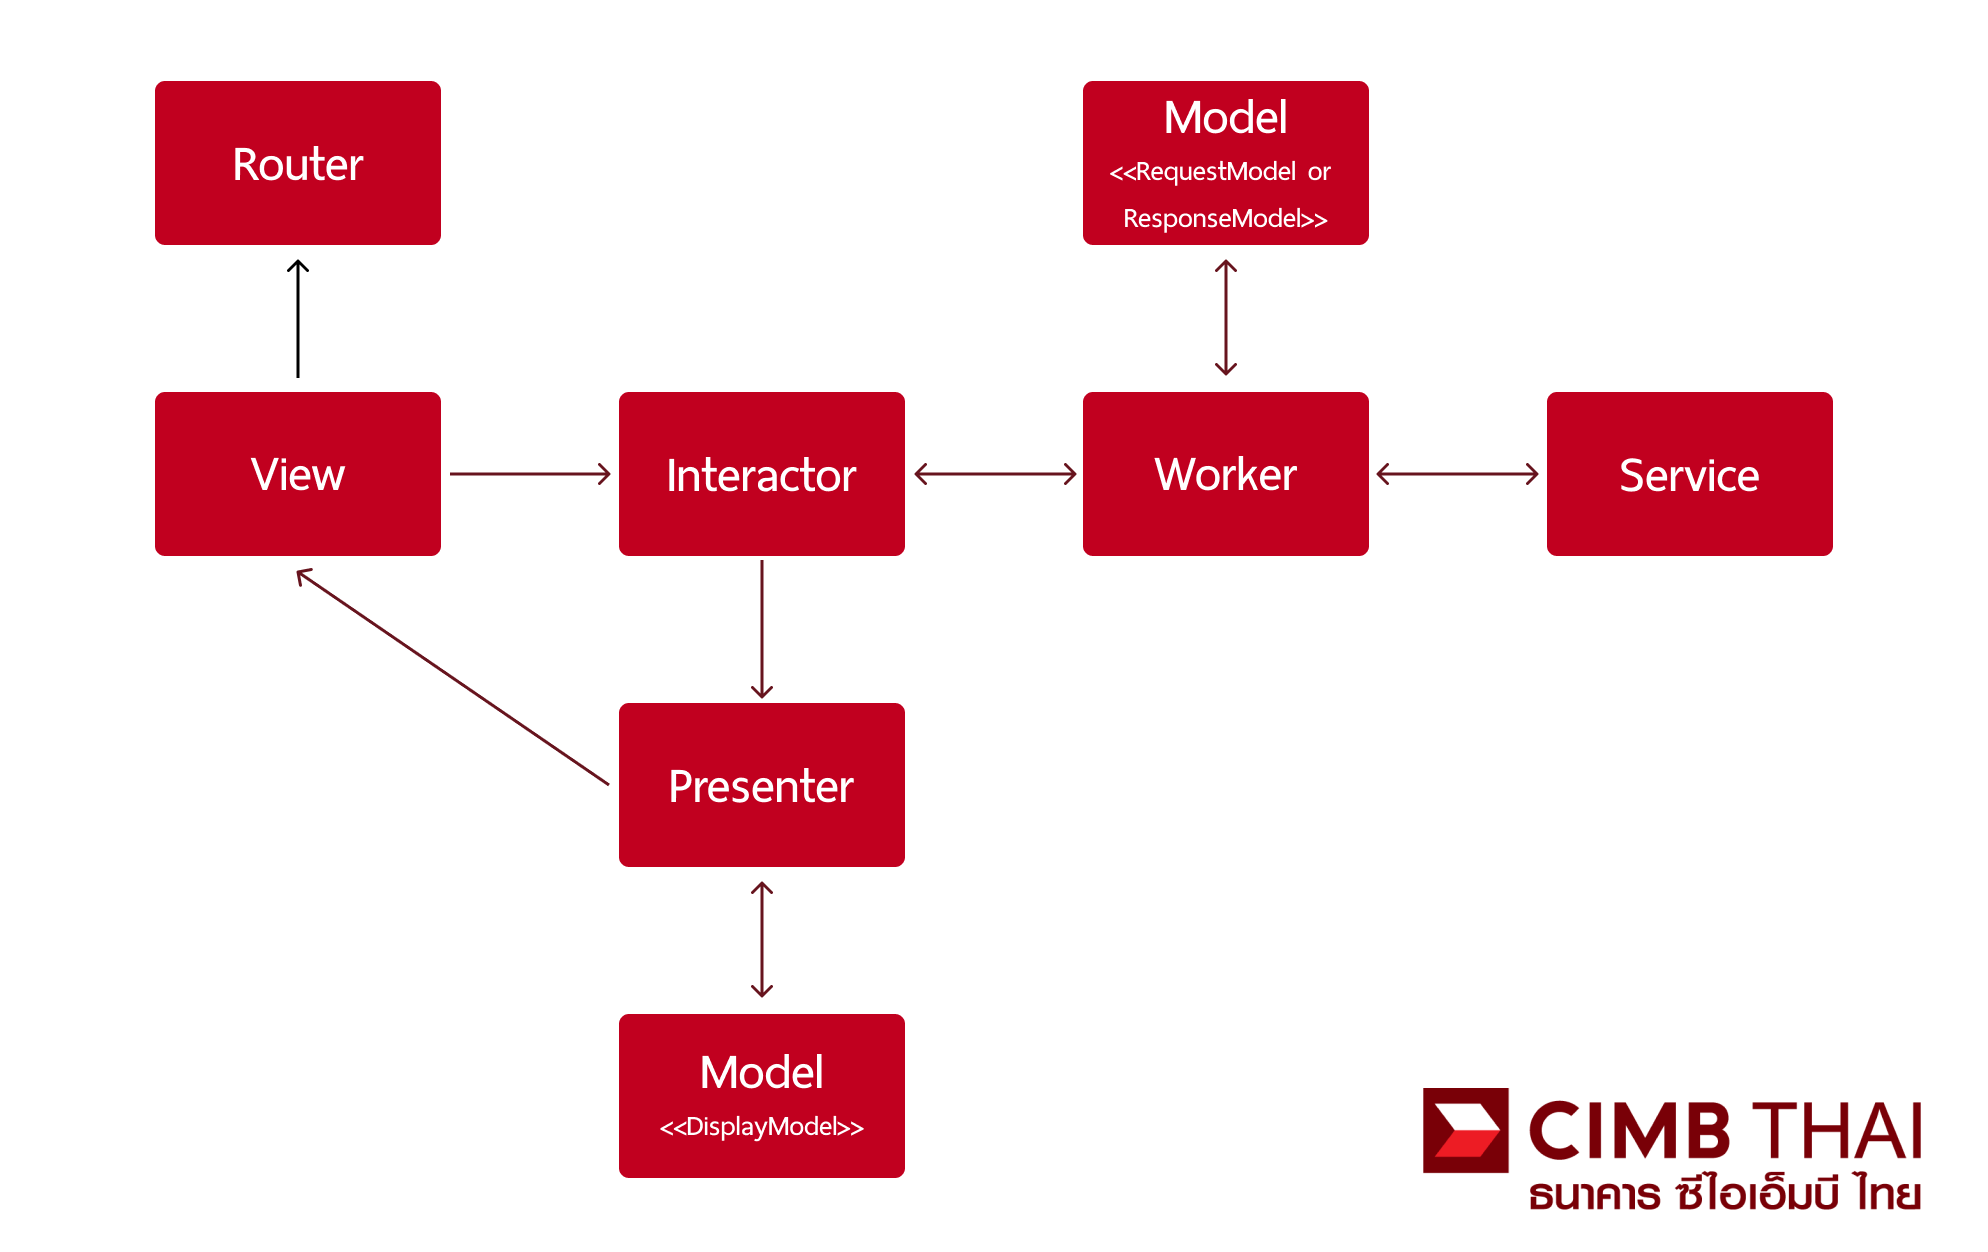
\includegraphics[width=1\textwidth]{vip-pattern}
%             \caption{รูปแบบการทำงานของ VIP}\label{vip-pattern}
%         \end{figure}
%         VIP คือรูปแบบในการพัฒนาซอฟต์แวร์รูปแบบหนึ่งที่แบ่งแยกการแสดงผล และส่วน Business Logic ออกจากกันโดยแยกออกมาหลัก ๆ ได้ 3 ส่วนคือ View, Interactor และ Presenter แต่ว่าจะมีส่วนแยกออกมาเพื่อทำงานให้สมบูรณ์อีกคือ Model, Router และ Worker
%         ซึ่งแต่ละส่วนนั้นทำงานดังนี้
%         \begin{enumerate}
%             \item \textbf{View} เป็นส่วนติดต่อลูกค้าที่จะคอยรับข้อมูลและแสดงผลให้ลูกค้า เมื่อมีข้อมูลเข้ามาจากลูกค้า Activity(Android) หรือ ViewController(iOS) เป็นคลาสที่คอยรับข้อมูลเพื่อส่งต่อให้ Interactor นำไปประมวลผลต่อ และแสดงผลโดยการนำข้อมูลที่จัดรูปแบบแล้วจาก Presenter มาแสดงผลให้กับลูกค้า
%             \item \textbf{Interactor} เป็นส่วนที่คอยรับการสั่งการมาจาก View เพื่อจัดเตรียมข้อมูล หรือคำนวณข้อมูลเพื่อที่จะส่งต่อไปยัง Presenter โดยข้อมูลนั้นจะมาจาก Worker ที่เป็นตัวส่งข้อมูลมาให้ เป็นที่ ๆ เกิด Business Logic ทุกอย่างที่นี่
%             \item \textbf{Worker} เป็นส่วนดึงข้อมูลจาก Service เพื่อนำมาใส่ Model ที่จัดเตรียมไว้เพื่ออยู่ในรูปแบบที่ใช้งานกับโค้ดทุก ๆ ส่วนในแอปพลิเคชันได้ หรือเป็นตัวสร้าง Request Model เพื่อร้องขอไปยัง Service
%             \item \textbf{Model (Response/Request)} เป็น Model ที่จะมีโครงสร้างเหมือน JSON ที่ได้รับการตอบรับมาจาก Service เพื่อที่จะสามารถนำข่้อมูลมาใส่ได้
%             \item \textbf{Service} เป็นส่วนที่ดึงข้อมูลจาก API เพื่อให้ได้การตอบรับแบบ JSON เพื่อที่จะส่งต่อไป Worker หรือนำข้อมูลที่ได้จาก Worker ส่งไปยัง API เพื่อร้องขอข้อมูล
%             \item \textbf{Presenter} เป็นส่วนที่จะคอยนำข้อมูลจาก Interactor มาจัดในรูปแบบที่จะแสดงผล หรือคือ DisplayModel เพื่อที่จะส่งไปให้กับ View ได้แสดงผล
%             \item \textbf{Model (Display)} เป็น Model ที่จะมีโครงสร้างตามลักษณะของส่วนติดต่อลูกค้า
%             \item \textbf{Router} เป็นส่วนที่คอยจัดการเรื่องการพาไปยังส่วนติดต่อลูกค้าในหน้าอื่น ๆ
%         \end{enumerate}

%     \subsection{Continuous Integration/Continuous Delivery (CI/CD)}
%     \textbf{Continuous Integration (CI)} คือ กระบวนท่าที่ใช้สำหรับการรวบรวมซอฟแวร์ที่มีการพัฒนาแยกส่วนกันอย่างอัตโนมัติ อาจจะโดยหนึ่งหรือหลายนักพัฒนาก็ตามที สุดท้ายแล้วซอฟแวร์ที่พัฒนาชิ้นเล็กๆ ที่พัฒนาขึ้นมาจะต้องนำมารวมกันเป็นชิ้นใหญ่หนึ่งชิ้น จะทำอย่างไรให้มั่นใจได้ว่า ไม่มีชิ้นส่วนใดที่จะส่งผลให้ชิ้นส่วนอื่นๆ พังเสียหาย เนื่องจากเป็นการพัฒนาโดยโปรแกรมเมอร์หลายคน
%     ซึ่งเป็นไปได้ว่าจะมี bug หลุดมาจากส่วนใดส่วนหนึ่ง แล้วเราจะป้องกันได้อย่างไรละ ดังนั้นจึงต้องมีการเขียน script test ที่คอยทดสอบความเข้ากันได้ของแต่ละชิ้นส่วนโดยอัตโนมัตินั่นเอง โดยการ Testing จะเริ่มตั้งแต่ Unit Testing ซึ่งสร้างจากทีมพัฒนา และเป็นส่วนจะใช้ตรวจสอบว่าสิ่งที่ทีมพัฒนายังทำงานถูกต้องและจะใช้เวลาช่วงสั้น ๆ เท่านั้น
%     โดยในโลกของการพัฒนานั้น มักใช้ Build Server มาช่วยเพื่อให้เป้าหมายที่ตั้งไว้สำเร็จ กล่าวคือ จะเริ่มทำการ Integration กันตั้งแต่เมื่อมีการเปลี่ยนแปลง Source Code ที่ Repository กลาง ระบบจะทำการตรวจสอบ Code หลังจากการเปลี่ยนแปลงว่าทำงานร่วมกันได้หรือไม่ตั้งแต่ Compile, Testing
    
%     ส่วน \textbf{CD} นั้นสามารถแบ่งได้สองประเภทตามวิธีการ Deploy ดังรูปที่ \ref{cd}
%     \begin{figure}[H]
%         \centering
%         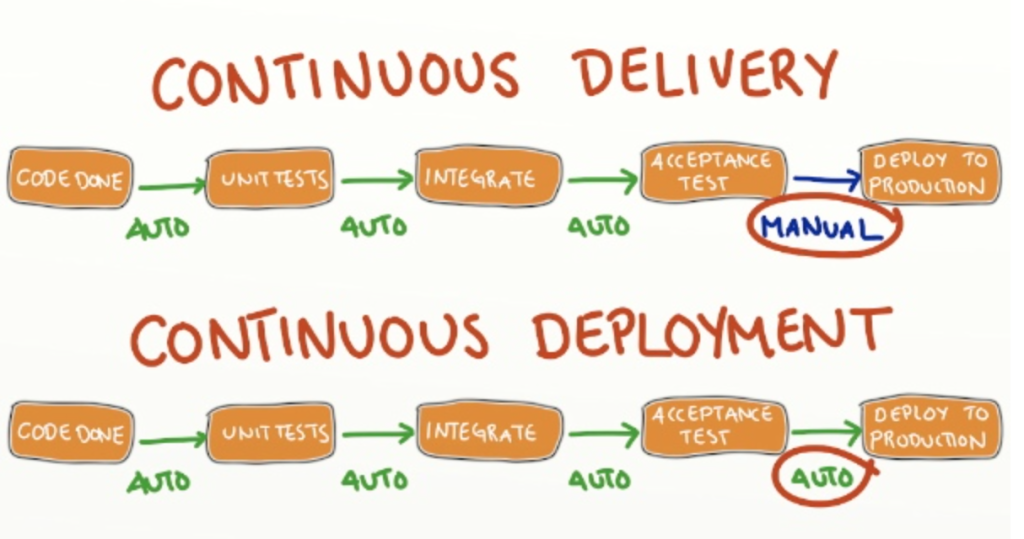
\includegraphics[width=1\textwidth]{cd}
%         \caption{ความแตกต่างของ Continuous Deployment และ Continuous Delivery }\label{cd}
%     \end{figure}
%     \begin{itemize}
%         \item[-] Continuous Deployment คือ ในทุกๆ ขั้นตอนจนถึงการ deployment ขึ้น production จะทำแบบอัตโนมัติทั้งหมด
%         \item[-] Continuous Delivery คือ การงานต่างๆ ใน deployment pipeline นั้น จะเริ่มต้นทำงานตั้งแต่การ compile, build ไปจนถึงขั้นตอนการทดสอบต่างๆ เช่น Acceptance test เป็นแบบอัตโนมัติทั้งหมด ส่วนในขั้นตอนการ deployment ขึ้น production นั้น จะต้องได้รับการอนุมัติหรือการตัดสินใจกันก่อนจากทาง Business ซึ่งเป็นการทำงานแบบ manual นั่นเอง หรืออาจจะเป็น One Click Deploy ก็ได้\cite{cicd}
%     \end{itemize}

% \section{เครื่องมือที่ใช้งาน}
%     \subsection{Android Studio}
%         \begin{figure}[H]
%             \centering
%             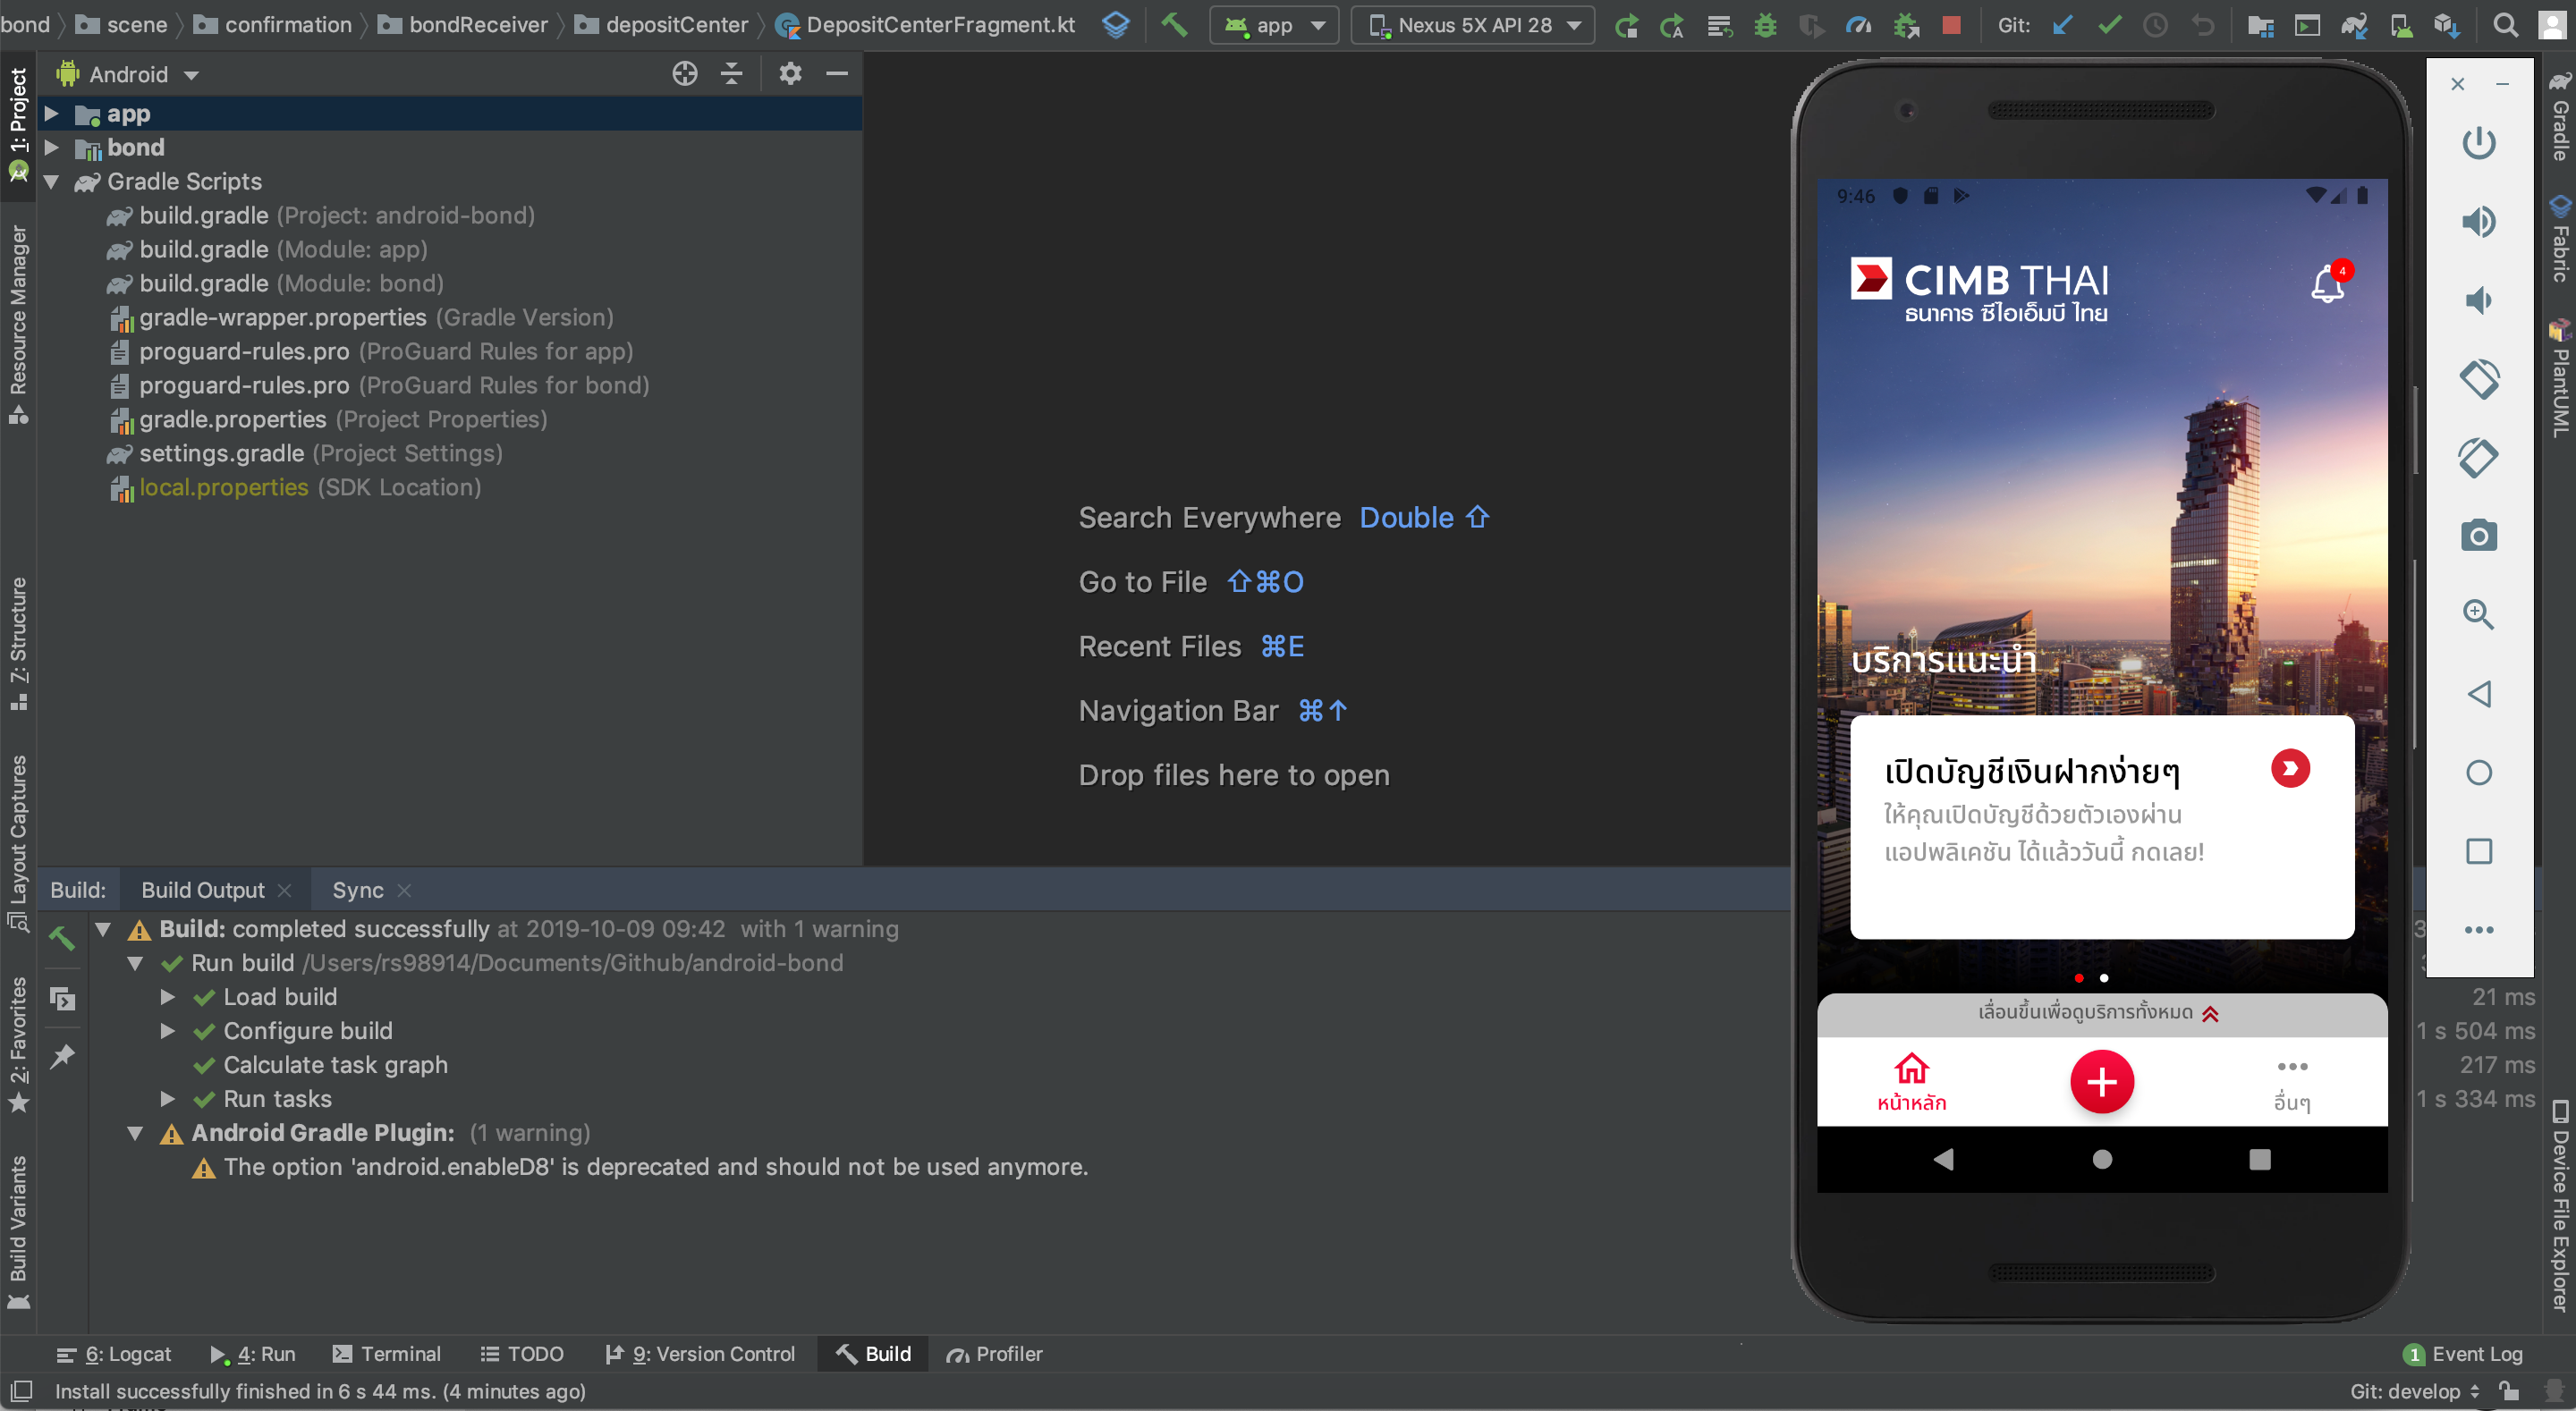
\includegraphics[width=1\textwidth]{android-studio}
%             \caption{หน้าการใช้งาน Android Studio}\label{android-studio}
%         \end{figure}
%         Android Studio คือเครื่องมือพัฒนา IDE (ไอ ดี อี) หรือ Integrated Development Environment (อินทิเกรต ดีเวลลอปเม้นท์ (เอนไวรอนเม้นท์) ที่ถูกสร้างขึ้นมาเพื่อการพัฒนาแอนดรอยด์แอปพลิเคชั่น บนพื้นฐานของแนวคิด InteliJ IDEA(อินเทล ไอ เจ ไอดีอีเอ) คล้าย ๆ กับการทำงานของ Eclipse (อีคิปส์)และ Android ADT Plugin (แอนดรอยด์ เอดีที ปลั๊กอิน) และเป็น IDE Tools (ไอ ดี เอ็ม ทูล) ล่าสุดจาก Google (กูเกิ้ล)  ไว้พัฒนาโปรแกรม Android (แอนดรอยด์)\cite{android-studio}

%     \subsection{Kotlin}
%         \begin{figure}[H]
%             \centering
%             
\includegraphics[width=0.5\textwidth]{kotlin-logo}
%             \caption{ตราสัญลักษณ์ภาษา Kotlin}\label{kotlin-logo}
%         \end{figure}
%         Kotlin คือภาษาโปรแกรมมิ่งที่ได้รวมหลักการเขียนโปรแกรมแบบเชิงวัตถุ และ หลักการเขียนโปรแกรมแบบฟังก์ชันเข้ามาร่วมกันซึ่งยังคงทำงานกับ JVM เช่นเดียวกับ Java แต่ได้เพิ่มความสามารถใหม่ที่ไม่มีใน Java และแก้ไขข้อผิดพลาดที่เกิดขึ้นใน Java รวมทั้ง Syntax ก็สั้นกระชับเข้าใจง่ายและมีความปลอดภัยสูง  เพราะ Kotlin จะเข้มงวดกับการประกาศประเภทของตัวแปรอย่างมาก โดยภาษา Kotlin ถูกพัฒนาโดยบริษัท JetBrains

%     \subsection{Xcode}
%         \begin{figure}[H]
%             \centering
%             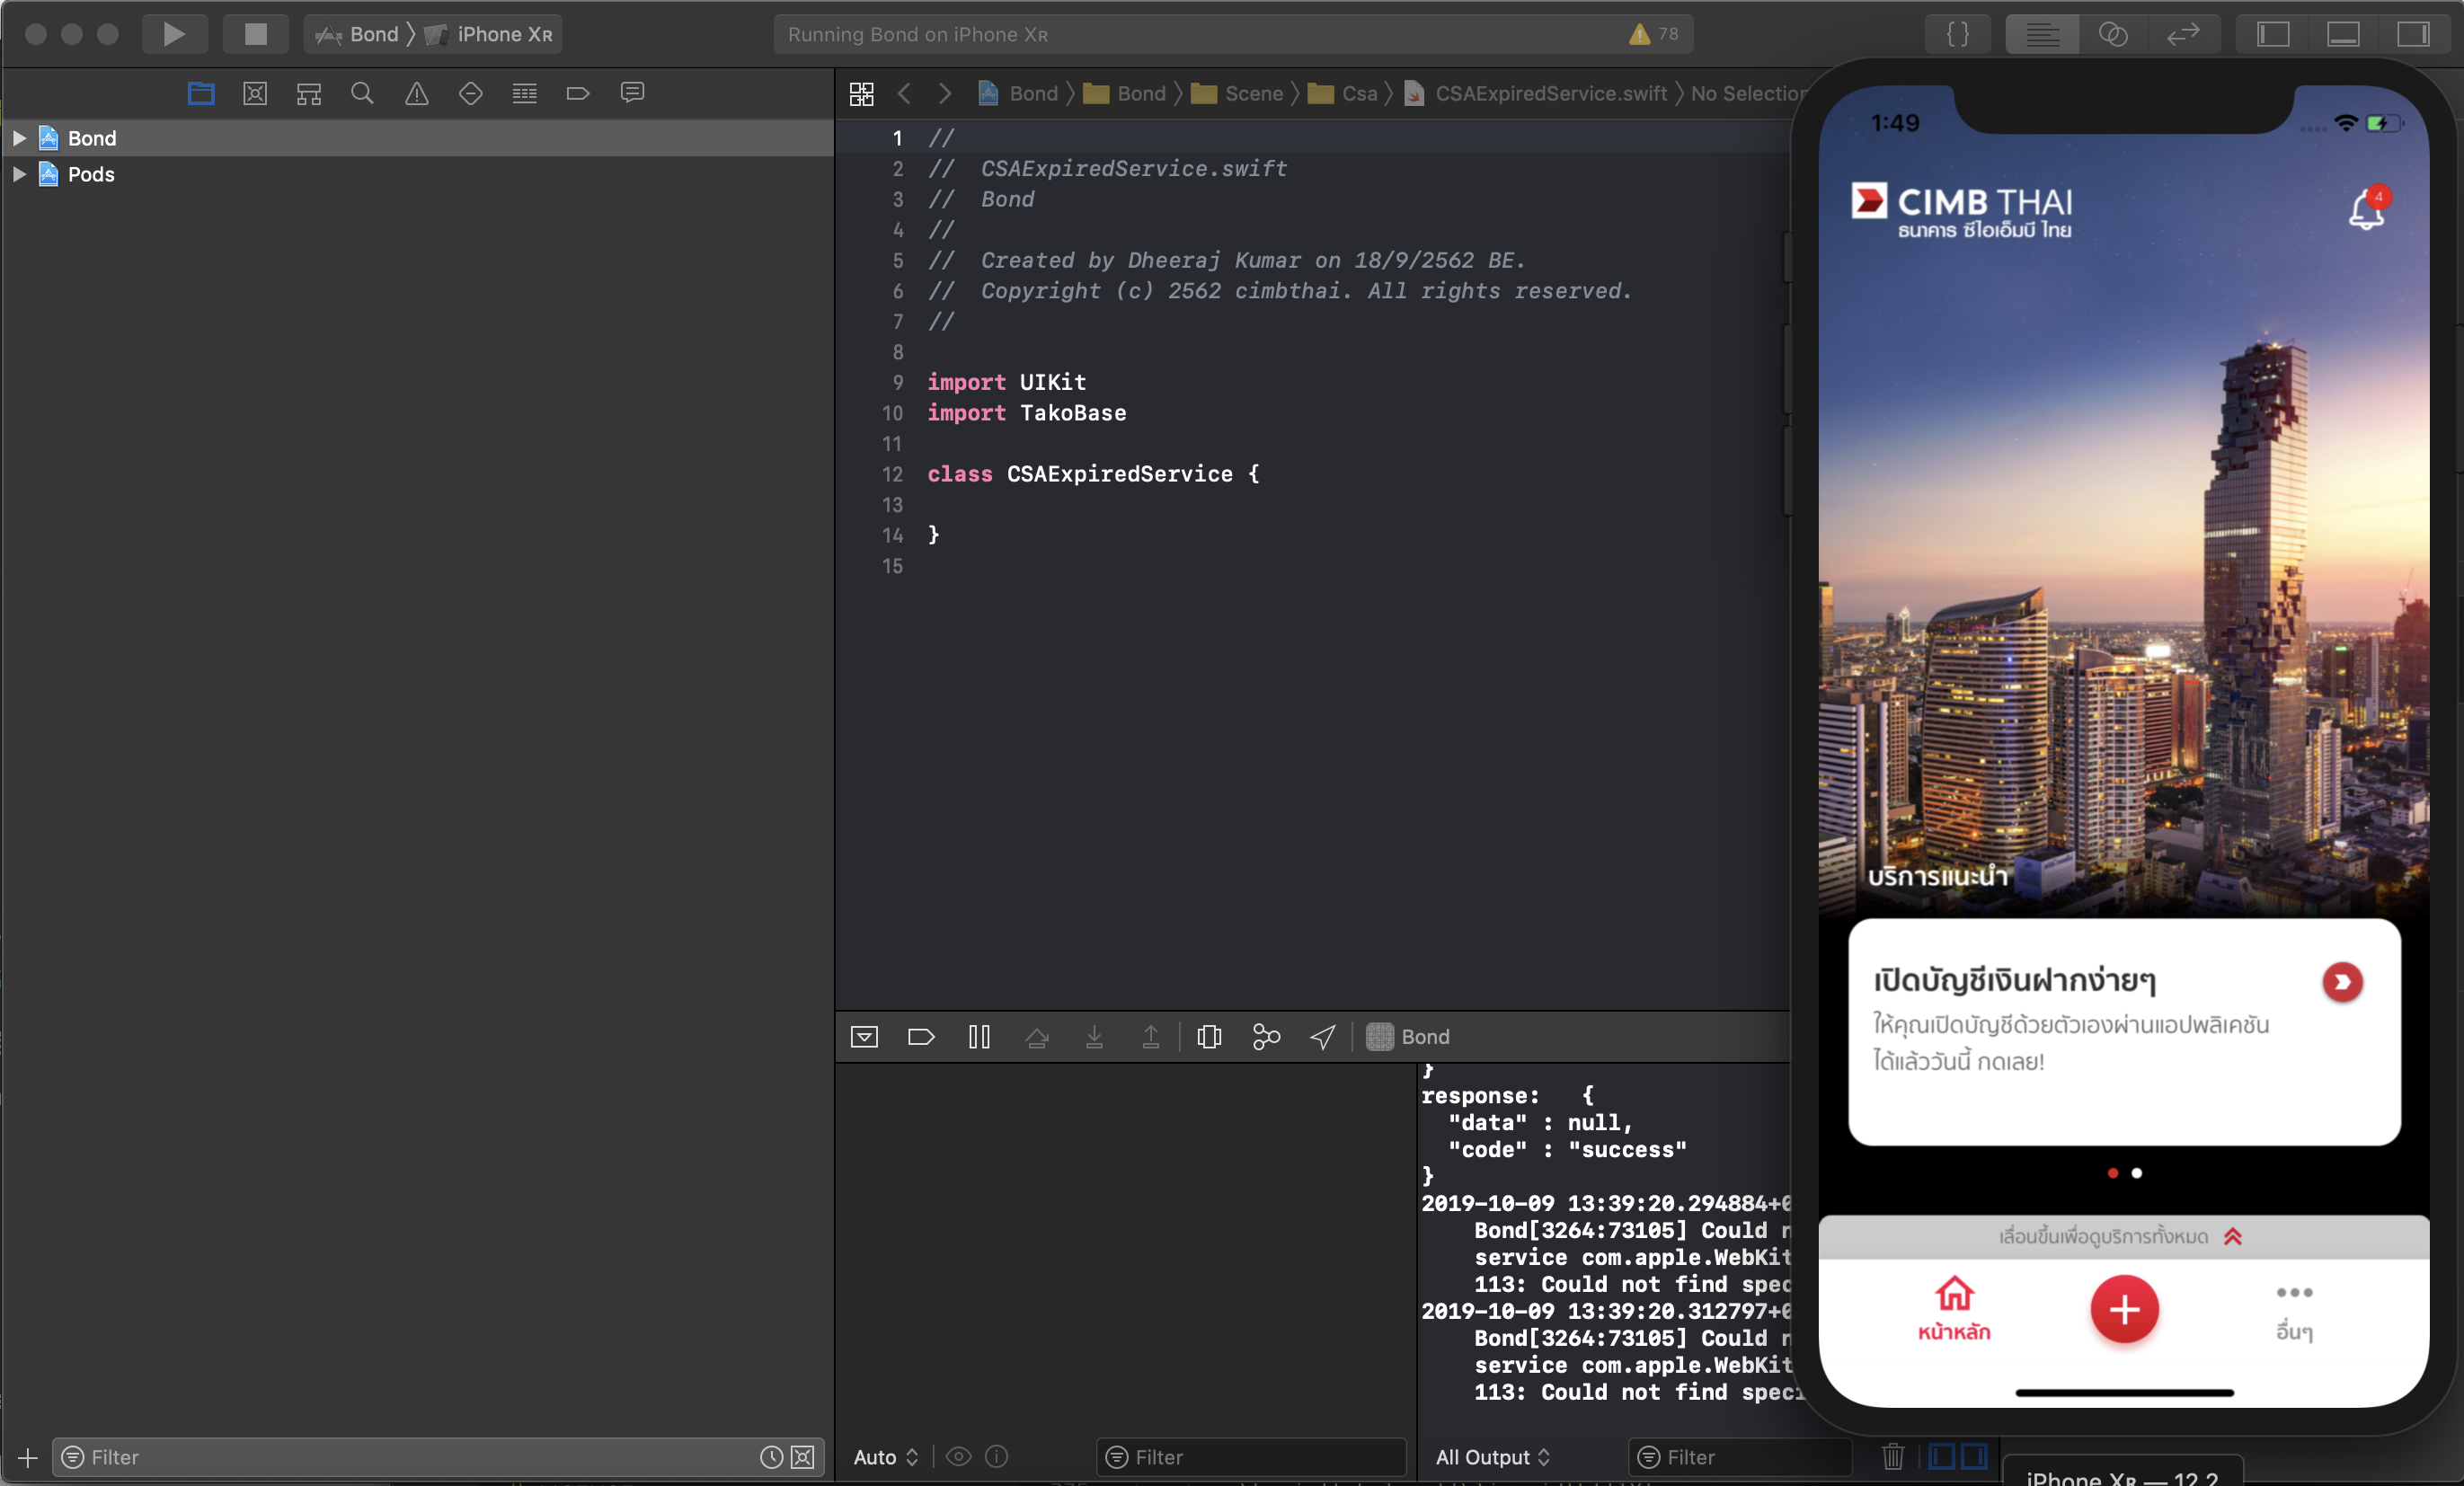
\includegraphics[width=1\textwidth]{xcode}
%             \caption{หน้าการใช้งาน Xcode}\label{xcode}
%         \end{figure}
%         Xcode คือเครื่องมือสำหรับนักพัฒนาโปรแกรม และแอปพลิเคชันบนแพลตฟอร์ม OS X และ iOS บนสมาร์ทโฟนที่ผลิตโดยบริษัท Apple

%     \subsection{Swift}
%         \begin{figure}[H]
%             \centering
%             
\includegraphics[width=0.5\textwidth]{swift-logo}
%             \caption{ตราสัญลักษณ์ภาษา Swift}\label{swift-logo}
%         \end{figure}
%         Swift คือภาษาโปรแกรมที่บริษัท Apple ได้สร้างและออกแบบมาเพื่อให้นักพัฒนาใช้พัฒนาโปรแกรมบน Mac OS X และ iOS โดยในอดีตจนถึงปัจจุบันภาษาที่ใช้คือ Objective-C โดยSwift เป็นภาษาที่ออกแบบให้มีประสิทธิภาพสูงและง่ายต่อการพัฒนาโดยนำข้อดีของภาษาสมัยใหม่เข้ามามากมาย เช่น Type Inference, Clean Syntax, No semicolons, Closures, Generics ซึ่งคุณสมบติที่กล่าวมาบางอย่างก็มีอยู่แล้วในภาษา Objective-C แต่ใน Swift นั้นจะน่าคบหามากขึ้น ภาษา Swift ยังถูกออกแบบให้มีความปลอดภัยในการเขียนโปรแกรมมากขึ้น\cite{swift}

%     \subsection{IntelliJ IDEA CE}
%         \begin{figure}[H]
%             \centering
%             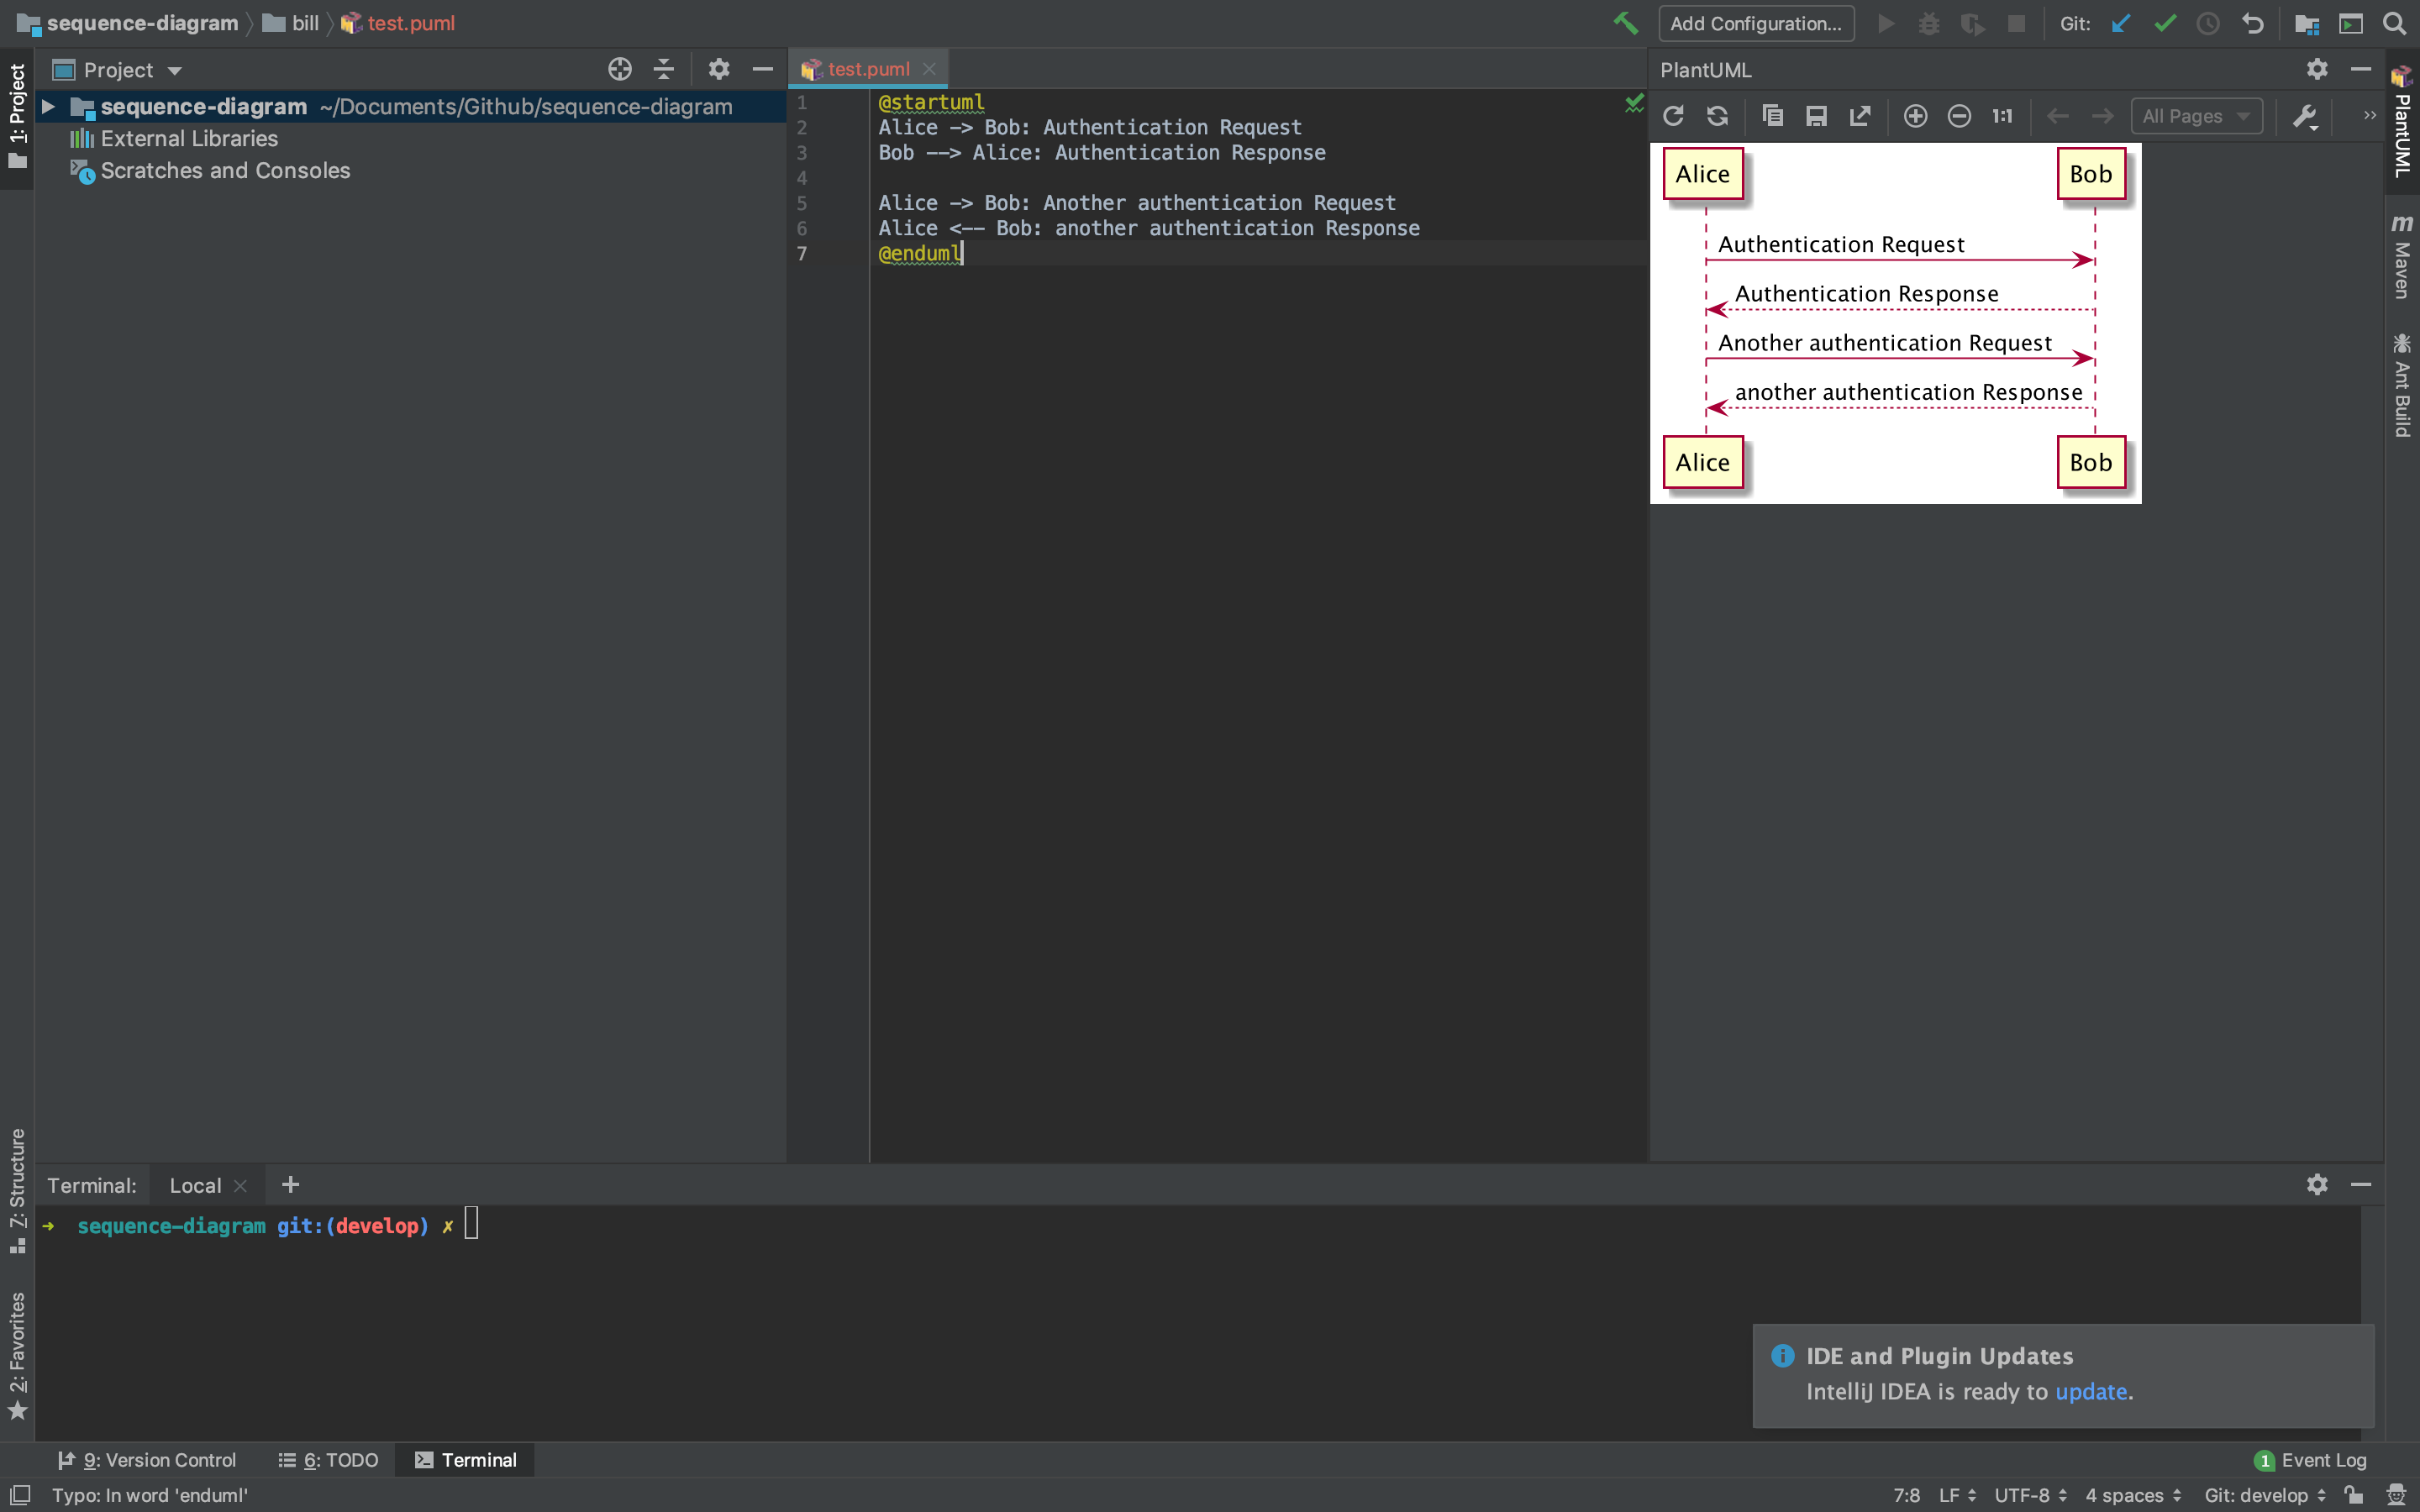
\includegraphics[width=1\textwidth]{intellij-idea}
%             \caption{หน้าการใช้งาน IntelliJ IDEA CE}\label{intellij-idea}
%         \end{figure}
%         IntelliJ IDEA CE คือเครื่องมือที่ช่วยในการพัฒนาโปรแกรมที่พื้นฐานการทำงานเพื่อภาษา Java ที่ถูกพัฒนาโดยบริษัท JetBrains ซึ่งมีสิ่งอำนวยความสะดวกต่างๆ เช่น คำสั่ง Compile, Run และจัด Format Code อัตโนมัติเป็นต้น

%     \subsection{Visual Studio Code}
%         \begin{figure}[H]
%             \centering
%             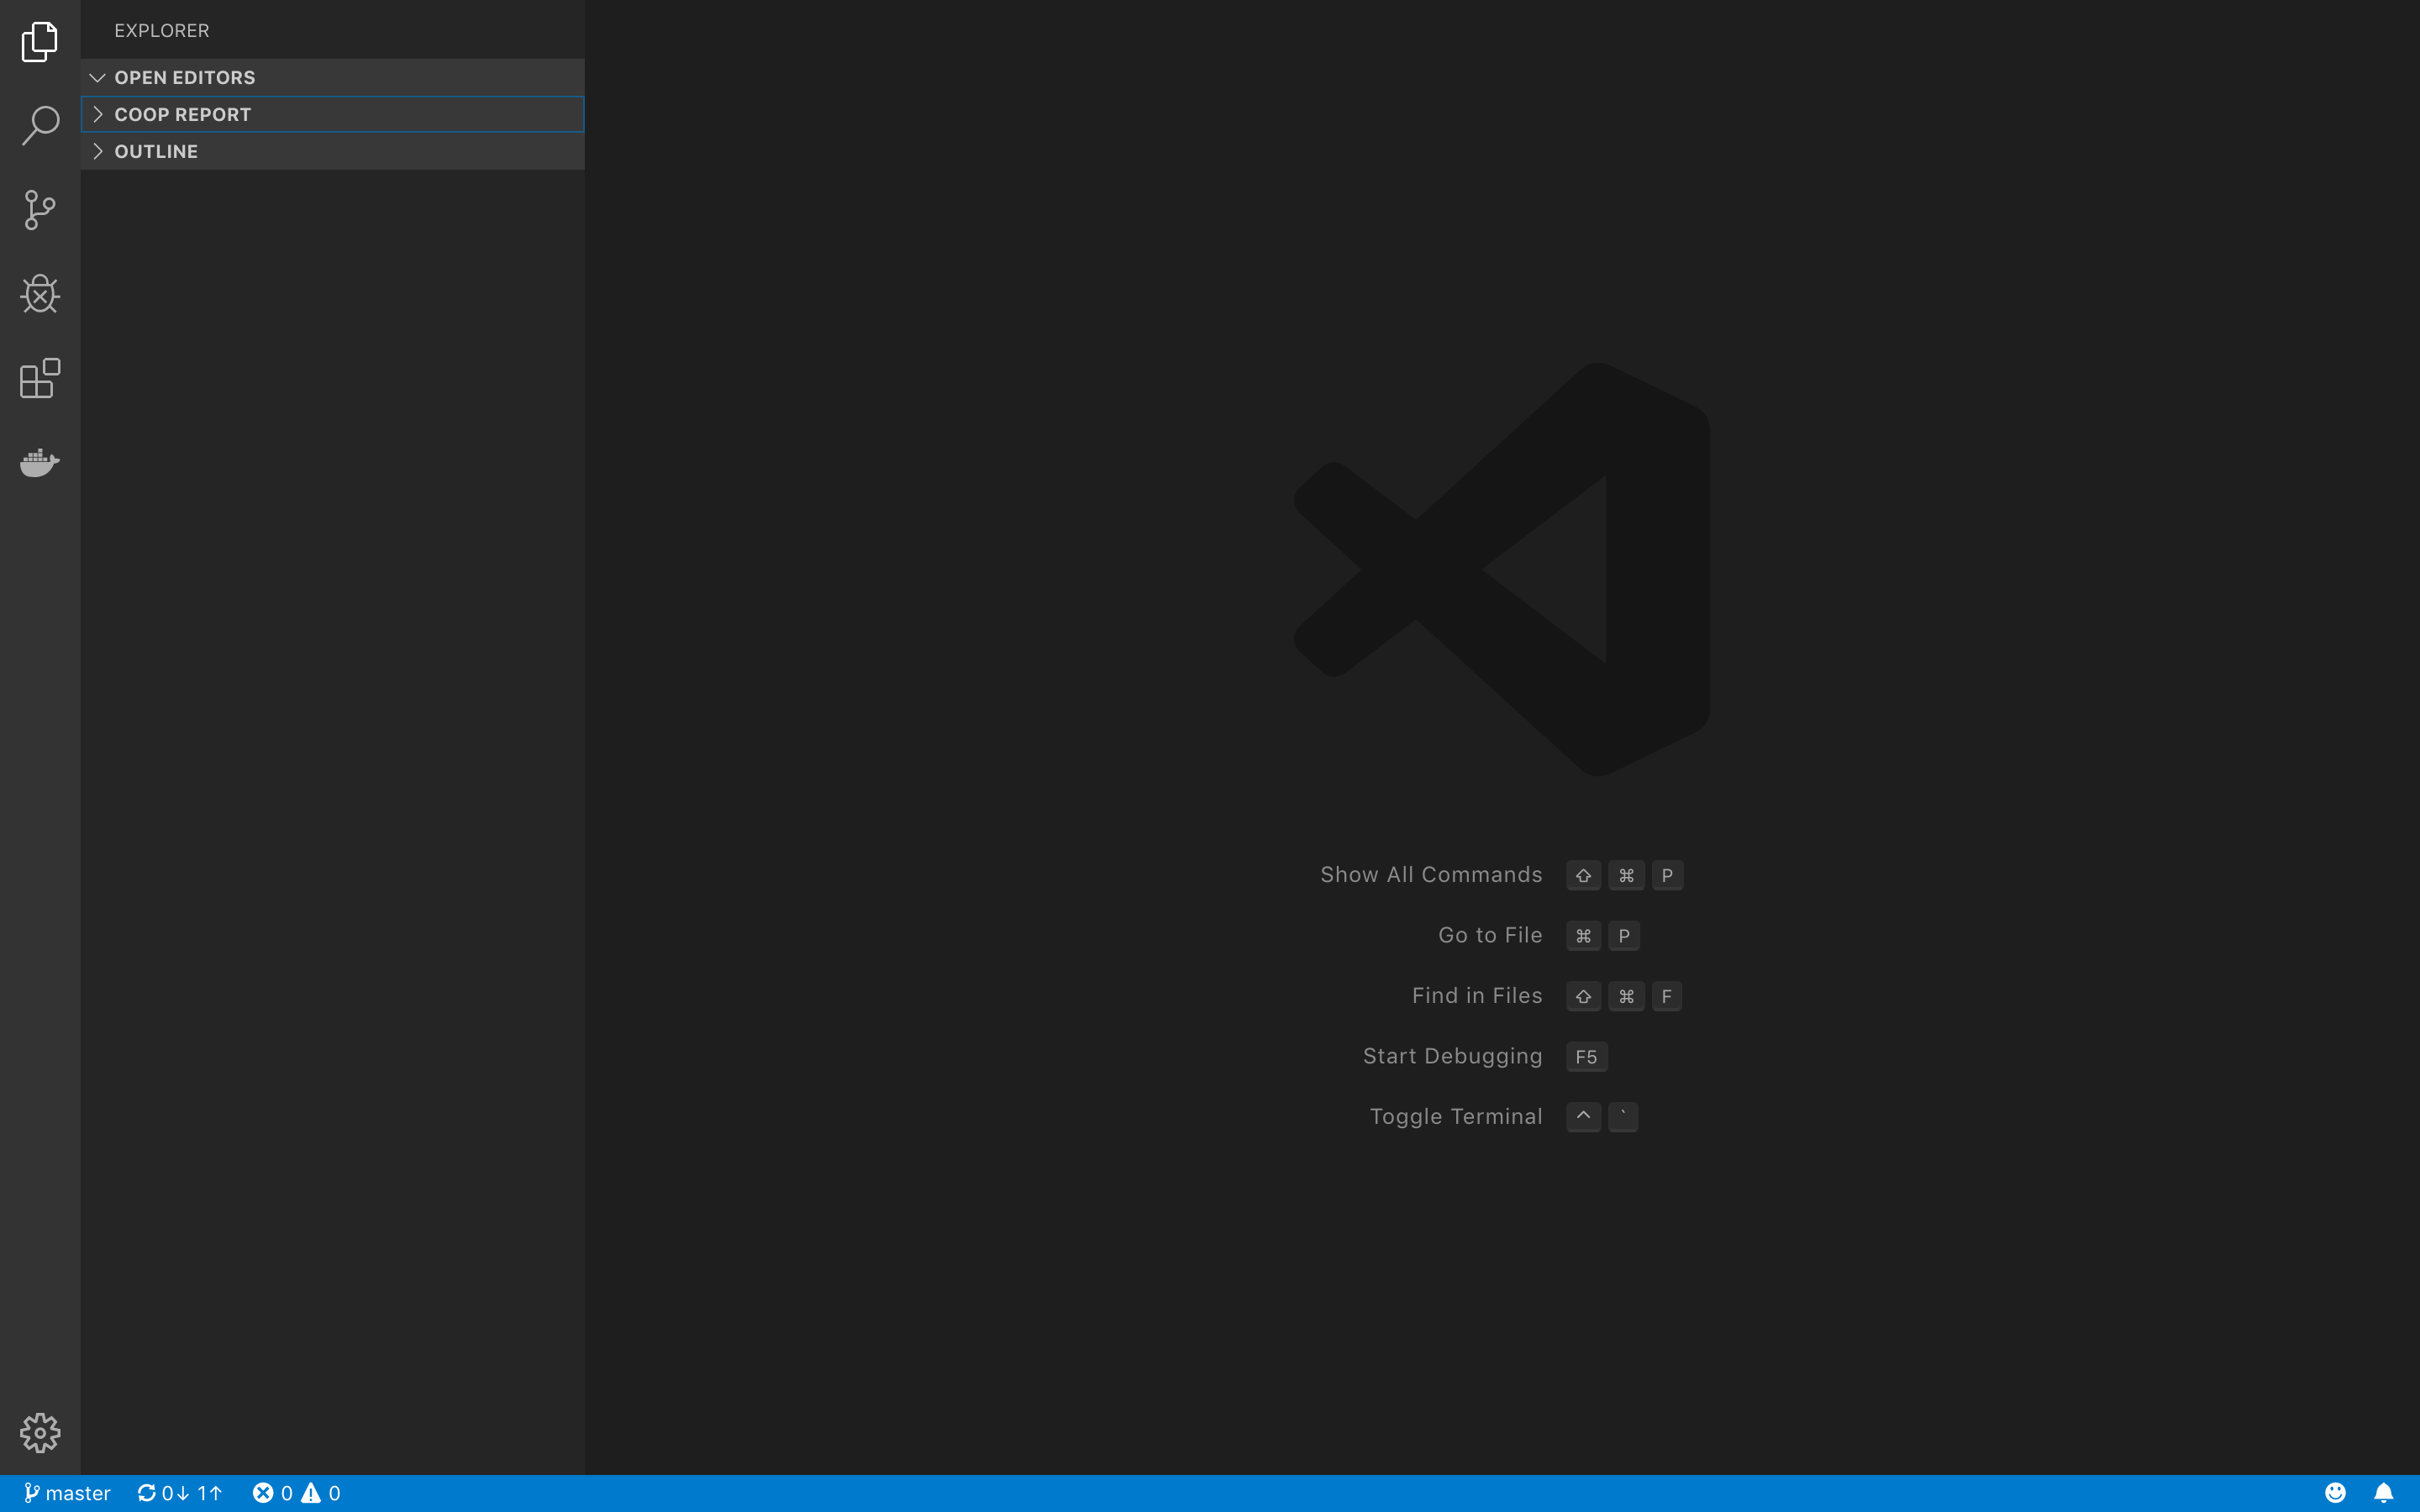
\includegraphics[width=1\textwidth]{visual-studio-code}
%             \caption{หน้าการใช้งาน Visual Studio Code}\label{visual-studio-code}
%         \end{figure}
%         Visual Studio คือโปรแกรม Code Editor ที่ใช้ในการแก้ไขและปรับแต่งโค้ด จากค่ายไมโครซอฟท์ มีการพัฒนาออกมาในรูปแบบของ OpenSource จึงสามารถนำมาใช้งานได้แบบฟรี ๆ ที่ต้องการความเป็นมืออาชีพ
%         ซึ่ง Visual Studio Code นั้น เหมาะสำหรับนักพัฒนาโปรแกรมที่ต้องการใช้งานข้ามแพลตฟอร์ม รองรับการใช้งานทั้งบน Windows, macOS และ Linux สนับสนุนทั้งภาษา JavaScript, TypeScript และ Node.js 
%         สามารถเชื่อมต่อกับ Git ได้ นำมาใช้งานได้ง่ายไม่ซับซ้อน มีเครื่องมือส่วนขยายต่าง ๆ ให้เลือกใช้อย่างมากมาก

%     \newpage
%     \subsection{Python}
%         \begin{figure}[H]
%             \centering
%             
\includegraphics[width=0.5\textwidth]{python-logo}
%             \caption{ตราสัญลักษณ์ภาษา Python}\label{python-logo}
%         \end{figure}
%         Python คือภาษาโปรแกรมคอมพิวเตอร์ระดับสูง โดยถูกออกแบบมาให้เป็นภาษาสคริปต์ที่อ่านง่าย  โดยตัดความซับซ้อนของโครงสร้างและไวยกรณ์ของภาษาออกไป ในส่วนของการแปลงชุดคำสั่งที่เราเขียนให้เป็นภาษาเครื่อง Python มีการทำงานแบบ Interpreter คือเป็นการแปลชุดคำสั่งทีละบรรทัด เพื่อป้อนเข้าสู่หน่วยประมวลผลให้คอมพิวเตอร์ทำงานตามที่เราต้องการ นอกจากนั้นภาษาโปรแกรม Python ยังสามารถนำไปใช้ในการเขียนโปรแกรมได้หลากหลายประเภท โดยไม่ได้จำกัดอยู่ที่งานเฉพาะทางใดทางหนึ่ง (General-purpose language) จึงทำให้มีการนำไปใช้กันแพร่หลายในหลายองค์กรใหญ่ระดับโลก

%     \subsection{Django}
%         \begin{figure}[H]
%             \centering
%             
\includegraphics[width=0.5\textwidth]{django-logo}
%             \caption{ตราสัญลักษณ์ภาษา Django}\label{django-logo}
%         \end{figure}
%         Python คือเป็นโครงร่าง Python Web ระดับสูงที่สนับสนุนการพัฒนาอย่างรวดเร็วและการออกแบบที่สะอาดและใช้งานได้จริง สร้างขึ้นโดยนักพัฒนาที่มีประสบการณ์ดูแลความยุ่งยากในการพัฒนาเว็บไซต์เป็นอย่างมากดังนั้นคุณจึงสามารถมุ่งเน้นไปที่การเขียนแอพของคุณโดยไม่จำเป็นต้องคิดค้นใหม่

%     \subsection{Vue.js}
%         \begin{figure}[H]
%             \centering
%             
\includegraphics[width=0.5\textwidth]{vue-logo}
%             \caption{ตราสัญลักษณ์ภาษา Vue.js}\label{vue-logo}
%         \end{figure}
%         Vue.js คือเป็น Progressive framework รูปแบบที่ถูกออกแบบมาให้จัดการ กับ UI โดยตัวหน้าที่หลักจะเน้นไปที่ส่วน View Layer เท่านั้น ด้วยการออกแบบที่ใช้งานได้ง่ายทำให้เหมาะสมกับการนำมาใช้ที่ส่วนๆ นึงใน Website หรือใช้กับทั้ง Website ได้เลยในรูปแบบของ Single Page Applcation 

%     \subsection{Git}
%         \begin{figure}[H]
%             \centering
%             
\includegraphics[width=0.5\textwidth]{git-logo}
%             \caption{ตราสัญลักษณ์ Git}\label{git-logo}
%         \end{figure}
%         Git คือ Version Control แบบ Distributed ตัวหนึ่ง เป็นระบบที่ใช้จัดเก็บและควบคุมการเปลี่ยนแปลงที่เกิดขึ้นกับไฟล์ชนิดใดก็ได้ ไม่ว่าจะเป็น Text File หรือ Binary File (จากนี้จะขอเรียก Text File หรือ Binary File รวมกันว่า Source Code)

%     \subsection{Hangouts Chat}
%         \begin{figure}[H]
%             \centering
%             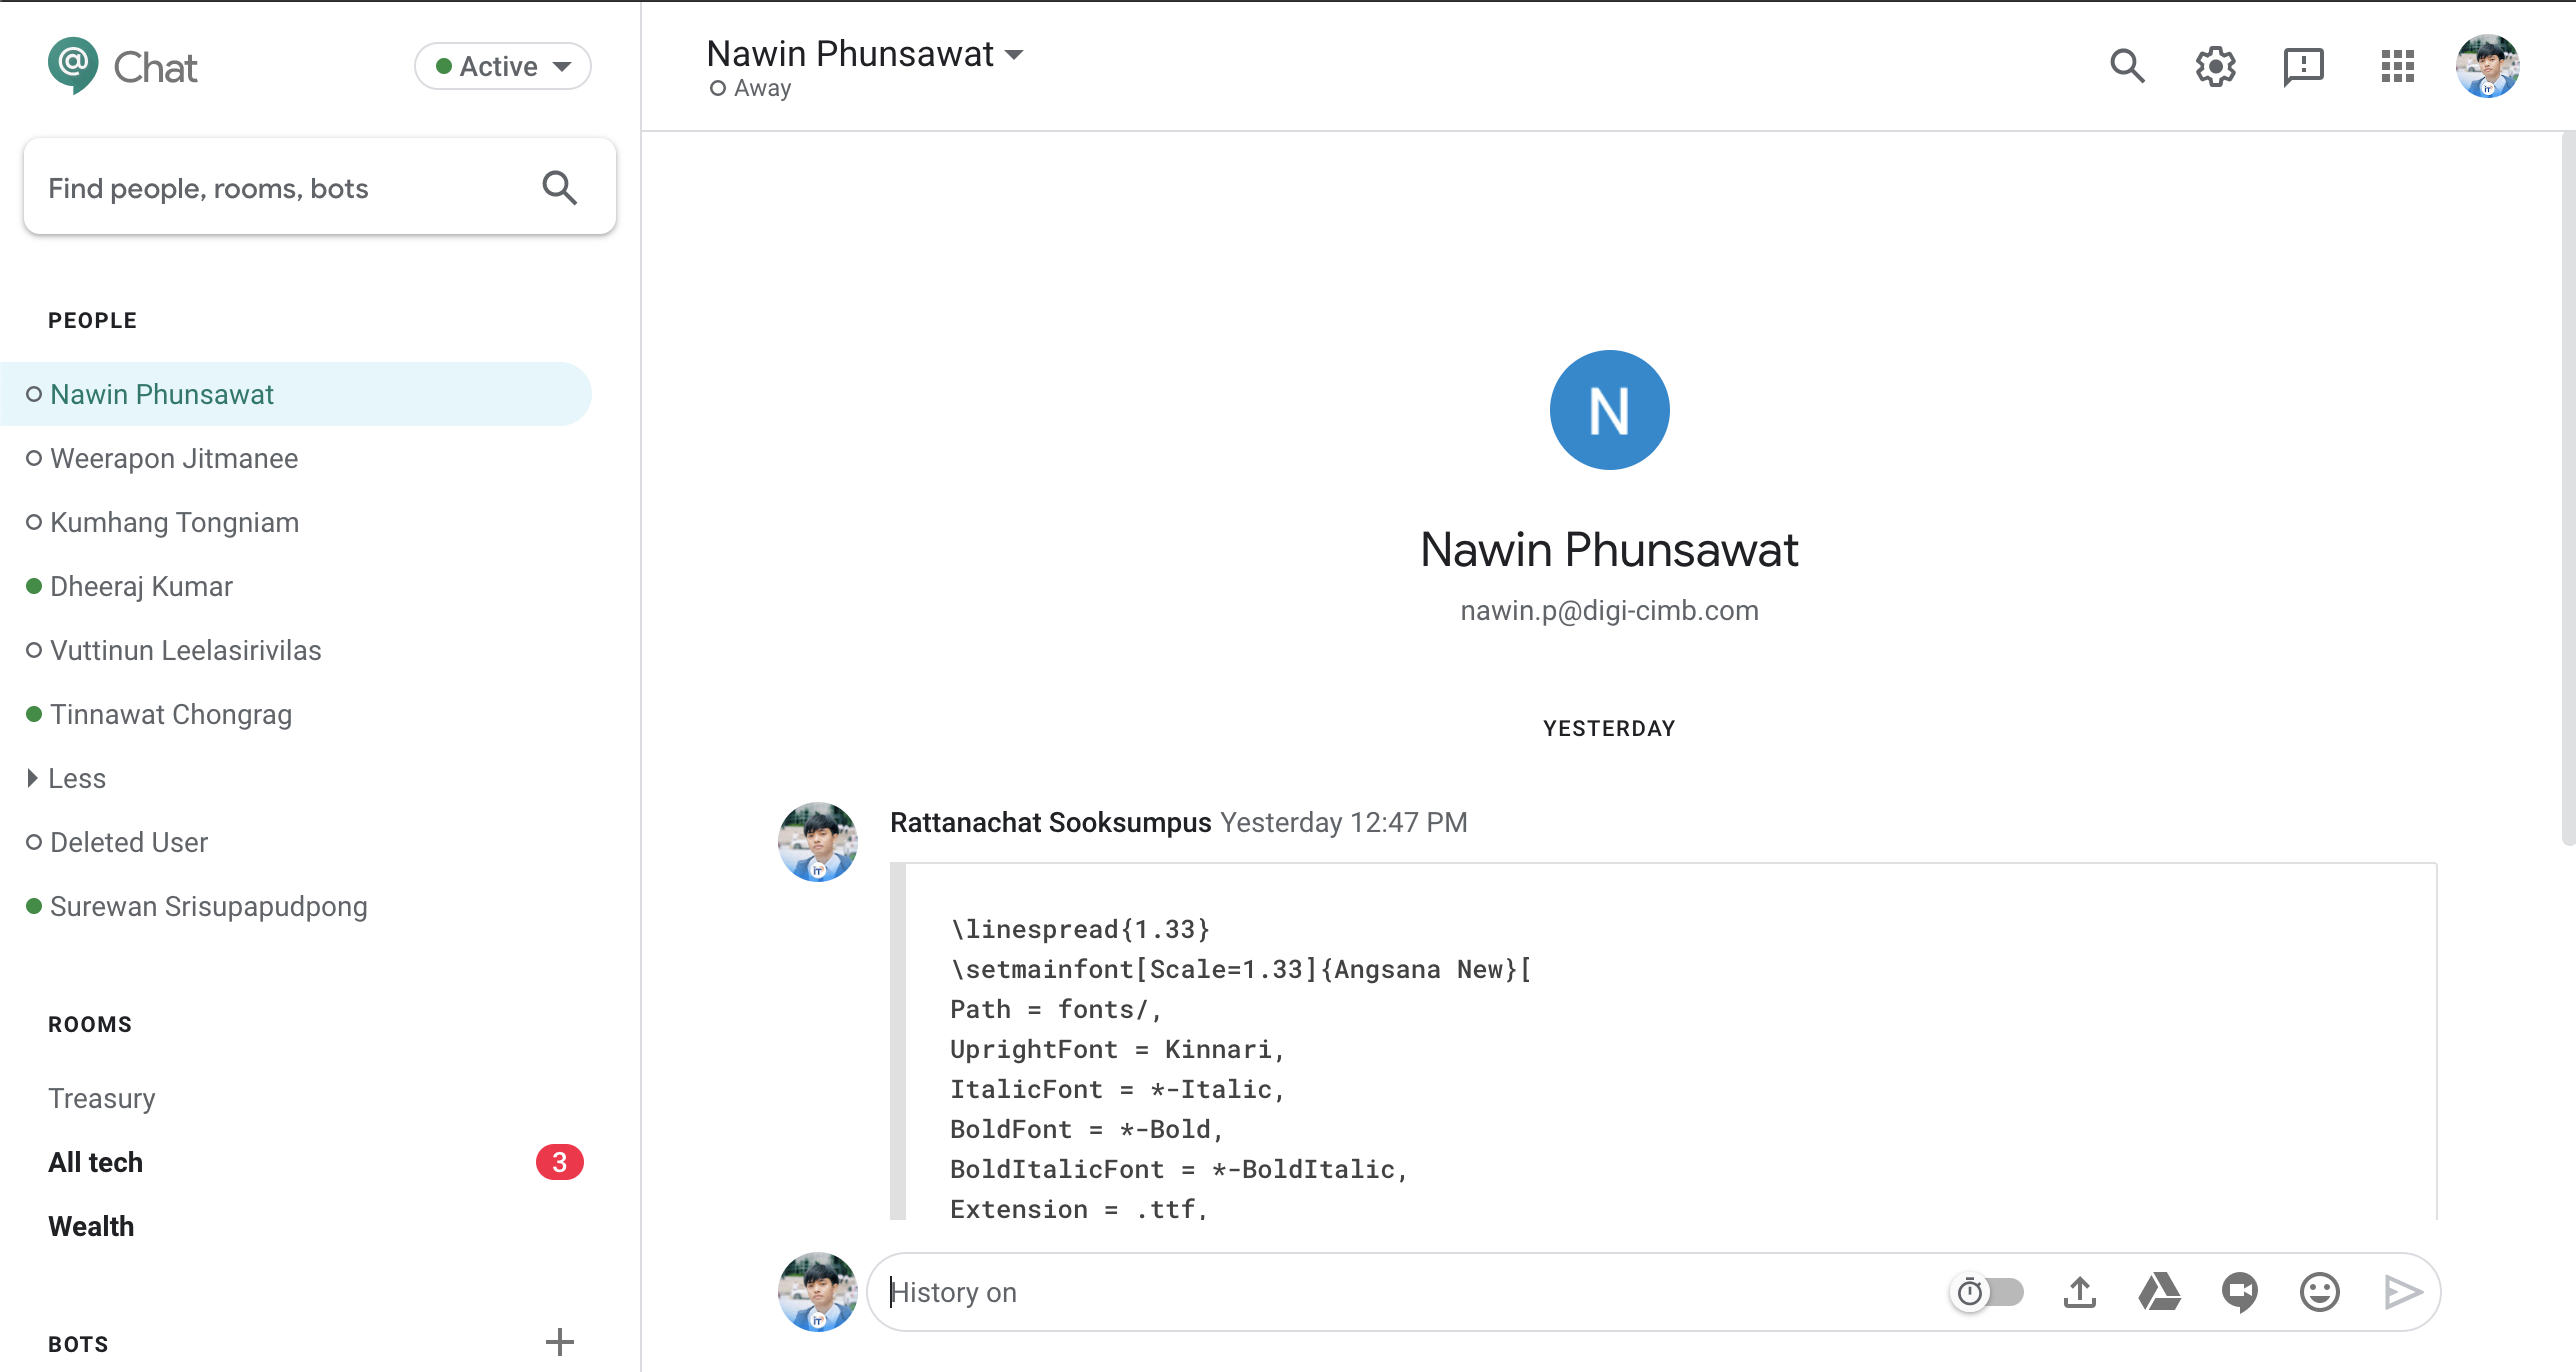
\includegraphics[width=1\textwidth]{chat}
%             \caption{หน้าการใช้งาน Hangouts Chat}\label{chat}
%         \end{figure}
%         Hangouts Chat คือแพลตฟอร์มการรับส่งข้อความที่สร้างขึ้นสำหรับทีม ทำให้ทีมทำงานได้ง่ายขึ้น ไม่ว่าจะเป็นการส่งข้อความส่วนตัวหรือข้อความกลุ่ม ช่วยให้ทีมทำงานร่วมกันได้อย่างคล่องตัวและมีประสิทธิภาพ อีกทั้งยังติดตามความคืบหน้าและผลการทำงานได้ง่ายด้วยห้องแชทออนไลน์เพื่อการทำงานร่วมกันและการสนทนาแบบเป็นชุดข้อความ ตอนนี้ Chat รองรับทั้งหมด 28 ภาษา ห้องแชทแต่ละห้องรองรับสมาชิกได้สูงสุด 8,000 คน

%     \subsection{Jira Software}
%         \begin{figure}[H]
%             \centering
%             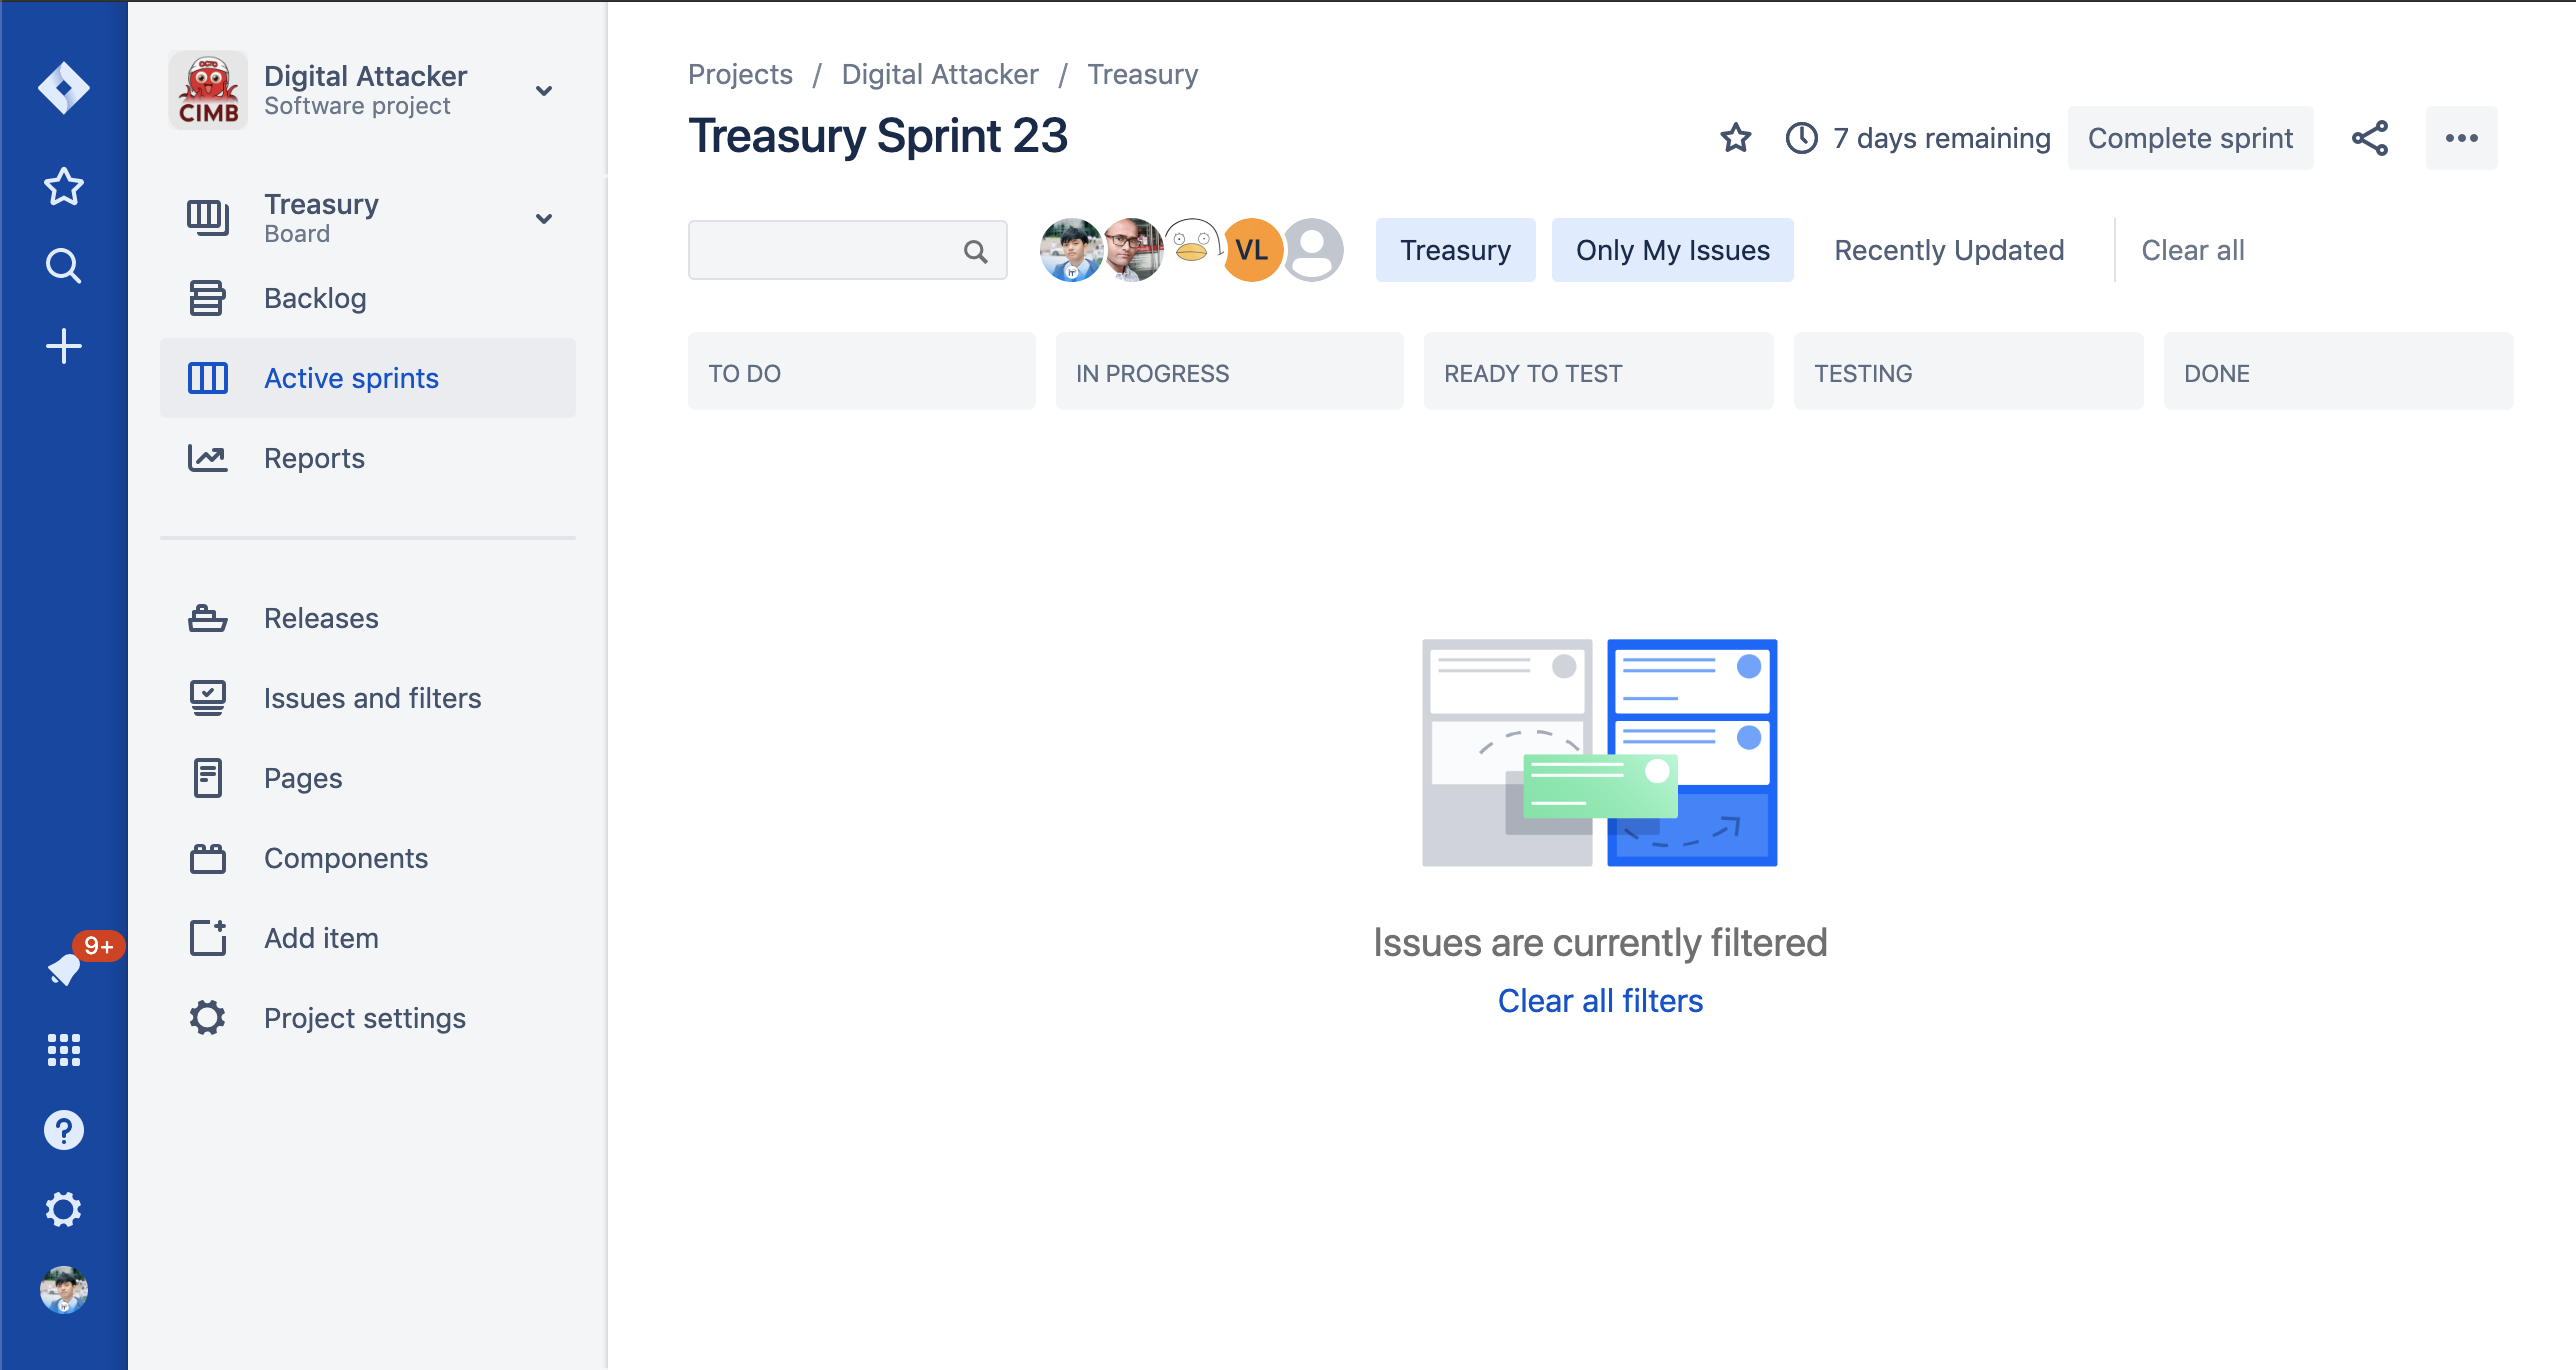
\includegraphics[width=1\textwidth]{jira}
%             \caption{หน้าการใช้งาน Jira Software}\label{jira}
%         \end{figure}
%         โปรแกรมติดตามและแก้ไขปัญหา โดยใช้หลักการของ Agile จัดทำขึ้นเพื่อใช้ในการแก้ไขความผิดพลาดของโปรแกรม (Bug) ติดตามปัญหา (Issue Tracking) และใช้ในการบริหารโครงการ (Project Management) พัฒนาโดยบริษัท Atlassion ข้อดีของโปรแกรมมีดังนี้
%         \begin{itemize}
%             \item[-] สามารถสร้างชิ้นงานได้ (Task) โดยสามารถกำหนดระยะเวลา (Estimate) หรือระดับความสำคัญ (Story Point) และสามารถมอบหมายงานให้แต่ละคนที่อยู่ในทีมได้
%             \item[-] สามารถแบ่งรอบการทำงานได้ (Sprint) ซึ่งในแต่ละรอบจะสามารถวางชิ้นงานได้ใน 5 ส่วนคือ งานที่ต้องทำ (To Do) งานที่กำลังดำเนินอยู่ (In Progress) งานที่พร้อมทดสอบ (Ready to Test) งานที่ที่กำลังทดสอบ (Testing) และงานที่เสร็จแล้ว (Done) โดยระหว่างที่รอบการทำงานยังไม่จบ สามารถที่จะลากชิ้นงานไปมาในได้ตลอด หากมีการแก้ไข
%             \item[-] เมื่อจบรอบการทำงานแล้ว จะมีแผนภูมิในแบบต่างๆ (Chart) สรุปผลการทำงานให้ ตามหลักของ Agile แล้ว นิยมใช้ Burndown Chart
%         \end{itemize}

%     \subsection{Jenkins}
%     \begin{figure}[H]
%         \centering
%         
\includegraphics[width=0.2\textwidth]{jenkins-logo}
%         \caption{ตราสัญลักษณ์ Jenkins}\label{jenkins-logo}
%     \end{figure}
%     Open Source Tools ที่ถูกเขียนด้วยภาษา Java ครับ โดย Jenkins ถูกสร้างขึ้นมาเพื่อตอบสนอง Concept 2 อย่างหลักๆ คือ 
%     Continuous integration และ Continuous Delivery โดยการรันเทสของเรานั้นจะเป็นการนำไปผูกอยู่กับ Flow ของ Continuous integration\cite{jenkins}

% \section{ลักษณะขั้นตอนการทำงาน}
% รูปแบบการทำงานใช้แบบ Agile โดยใช้โครงสร้างการทำงานแบบ Scrum ซึ่งก็คือทำเป็นวงรอบ (Sprint) ซึ่งแต่ละ Sprint จะมีระยะเวลา 3 สัปดาห์ โดยในแต่ละ Sprint จะรายละเอียดการทำงานดังนี้
% \subsection{Product Backlog Grooming}
% เป็นวันแรกของสัปดาห์ที่หนึ่งที่ทุก ๆ คนในทีมมาดูว่าใน Product Backlog มีงาน(Story)อะไรบ้างแล้วรายละเอียดแต่ละงาน(Story)เป็นยังไงมีส่วนไหนต้องทำบ้างไม่ว่าจะเป็น Frontend หรือ Backend โดยจะมีการ Estimate แต้มกันจนกว่าทุกคนจะให้แต้มเท่ากันโดยแต้มมีลำดับการให้เป็นลำดับ Fibonacci ถ้าให้ไม่เท่ากันก็จะถามเหตุผลในการให้แต้ม แล้ว Re-Estimate กันใหม่จนแต้มเท่ากันทุกคน

%     \subsection{Sprint Planning}
%     เป็นวันที่สองของสัปดาห์ที่นักพัฒนาจะทำการออกแบบ Sequence Diagram ของ Backend ว่าจะติดต่อกับ Mobile ยังไงแล้ว Flow แต่ละ Flow จะมี Request, Response อะไรบ้าง และมีการ Planning ในส่วนของ UI ที่ซับซ้อนเพื่อที่จะได้รองรับกรณี Error ได้ทั่วถึง 
        
%     \subsection{Develop And Test}
%     เป็นวันเริ่ม Sprint ที่ นักพัฒนาสามารถเริ่มต้นพัฒนาแอปพลิเคชันได้โดยการพัฒนานั้นนักพัฒนาคนนั้น ๆ ต้องทำการสร้างชุดทดสอบของส่วนที่ตัวเองนั้นพัฒนาด้วยโดยจะเริ่มตั้งวันที่สามของ Sprint ไปจนถึงวันสุดท้ายของสัปดาห์ที่สองโดยผู้ทดสอบแอปพลิเคชันระหว่างพัฒนาอยู่คือ Quality Assurance เพื่อหาจุดผิดพลาด(Bug) แล้วแจ้งนักพัฒนาแก้ไข

%     \subsection{Daily Stand-up}
%     เป็นกิจกรรมที่จะมีการมาอัพเดทงานและปัญหาที่เจอในวันก่อน ๆ และบอกสิ่งที่จะทำในวันนี้ซึ่งจะทำในทุก ๆ เช้าของวันทำงาน

%     \subsection{Product Backlog Refinement}
%     เป็นวันแรกของสัปดาห์ที่สองที่หัวหน้านักพัฒนาจะไปคุยว่างาน Sprint นี้สามารถทำทันไหมแล้วต้องการเอางานออกหรือเข้าตามความหมาะสม

%     \subsection{Sprint Review}
%     เป็นวันที่ 2 ของสัปดาห์ที่สามที่นักพัฒนามาสาธิตในงานที่ทำใน Sprint นี้หลังจากที่พัฒนา และทดสอบแล้วให้กับ Product Owner (PO) และ Project Manager (PM) เพื่อที่จะให้ PO และ PM ไปนำเสนอแอปพลิเคชันที่พัฒนาใน Sprint นี้กับทีม Business เพื่อให้ทีม Business ดูว่าตรงตามความต้องการมากน้อยแค่ไหน
    
%     \subsection{Release Code Day}
%     เป็นวันที่นักพัฒนาจะทำการอัปโหลดหรือปล่อยแอปพลิเคชันที่ทำใน Sprint นี่ขึ้นสู่สภาพแวดล้อม และ Server ของ User Acceptance Testing
    
%     \subsection{User Acceptance Testing}
%     User Acceptance Testing: เป็นวันที่ Quality Assurance หรือ QA จะทำการทดสอบแอปพลิเคชันโดยการจำลองเป็นลูกค้าแล้วหาจุดผิดพลาดเพื่อให้นักพัฒนาแก้ไขโดยจะเริ่มตั้งแต่วันที่ 3 ของสัปดาห์ที่สามจนถึงวันสุดท้ายของสัปดาห์ที่สาม

%     \subsection{PI Planning}
%     เป็นวันใดวันหนึ่งก็ได้ใน Sprint ที่หัวหน้านักพัฒนาจะคุยกับ Product Owner ถึง Product Backlog ใน Sprint ว่าจะต้องทำอะไรบ้างความต่้องการทางธุรกิจที่ไปเจรจาและรวบรวมมาจากทีม Business
            
%     \subsection{Sprint Retrospective}
%     เป็นวันสุดท้ายของสัปดาห์ที่สามที่ทุก ๆ คนในทีมไม่ว่าจะเป็น นักพัฒนา, หัวหน้านักพัฒนา, Quality Assurance, Project Manager และ Product Owner จะมาพูดถึงเรื่องราวต่าง ๆ ที่เกิดขึ้นใน Sprint ที่ผ่านมาไม่ว่าจะเป็นเรื่องงาน หรือเรื่องความเป็นอยู่ของคนในทีมโดยทาง Digital Banking จะเลือกใช้รูปแบบการ Retrospective เป็น Good, Bad, Try และ Next Action เพื่อที่จะมาบอกว่ามีอะไรบ้างที่ถือเป็นเรื่องดีไม่ดีใน Sprint นี้และมีอะไรที่ต้องพยายามให้มากขึ้นใน Sprint ถัดไปแล้ว Facilitator จะเป็นคนให้คนในทีมโหวตเพื่อเลือก Next Action มาสองอย่างจากเรื่องที่มีคนโหวตมากที่สุด

